\documentclass[a4paper, 11pt]{article}

\usepackage[utf8]{inputenc}
\usepackage[T1]{fontenc}
\usepackage[english]{babel}
\usepackage{enumitem}
\usepackage{amsthm, amsmath, amssymb, amsfonts, mathtools, mathrsfs}
\usepackage{graphicx, calc}
\usepackage{empheq}
\usepackage{geometry}
\geometry{a4paper, left = 20mm, right = 20mm, top = 30mm, bottom = 30mm}
\usepackage{xspace}
\usepackage{relsize}
\usepackage{fancyhdr}
\usepackage{pdflscape}
\usepackage{csquotes}
\usepackage{titling}
\usepackage{accents}
\usepackage[labelfont=bf,labelsep=period]{caption}
\usepackage{subcaption}
\usepackage{placeins} % FloatBarrier
\usepackage{physics}
\usepackage{tikz,tikz-3dplot}
\usetikzlibrary{patterns,decorations,decorations.markings}
\usepackage{lmodern}
\usepackage{xcolor}
\usepackage{booktabs}
\usepackage{chngcntr}
\usepackage{algorithm}
\usepackage{algorithmicx}
\usepackage{algpseudocode}
\usepackage[sorting=none, style=numeric]{biblatex}
\addbibresource{references.bib}


\usepackage{hyperref}
\hypersetup{
	colorlinks,
	citecolor=green,
	filecolor=black,
	linkcolor=blue,
	urlcolor=blue
}


\pagestyle{fancy}
\fancyhf{}
\setlength{\headheight}{30pt}
\lhead{Numerical Solution of the Convection--Diffusion Equations}
\rhead{ESEIAAT 2020--2021}
\cfoot{\thepage}

\setlength{\parskip}{0.2cm}%

% Comandos
\newcommand{\n}{\mathbb{N}}
\newcommand{\z}{\mathbb{Z}}
\newcommand{\q}{\mathbb{Q}}
\renewcommand{\real}{\mathbb{R}}
\newcommand{\cplex}{\mathbb{C}}
\renewcommand{\k}{\mathbb{K}}
\newcommand{\car}[1]{\mathrm{char}\left(#1\right)}
\newcommand{\class}[1]{\overline{#1}}
\newcommand{\mcd}[1]{\mathrm{mcd}{#1}}
\renewcommand{\mod}[1]{\ (\mathrm{mod}\ #1)}
\newcommand{\fractions}[1]{\mathrm{Fr}(#1)}
\renewcommand{\gcd}[1]{\mathrm{mcd} #1}
\newcommand{\mcm}[1]{\mathrm{mcm} #1}
\newcommand{\conj}[1]{\overline{#1}}
\newcommand{\prob}[1]{p \left( #1 \right)}
\newcommand{\esp}[1]{\mathbb{E} \left[ #1 \right]}
\newcommand{\scr}[2]{\left\langle #1, #2 \right\rangle}
\newcommand{\Int}{\int\limits}
\newcommand{\id}{\mathrm{Id}}
\newcommand{\lt}[1]{\mathrm{LT}(#1)}
\newcommand{\lc}[1]{\mathrm{LC}(#1)}

\newcommand{\divides}{\mid}
\newcommand{\notdivides}{\nmid}
\newcommand{\MATLAB}{\textsc{Matlab}\xspace}
\newcommand{\CC}{C\nolinebreak[4]\hspace{-.05em}\raisebox{.4ex}{\relsize{-3}{\textbf{++}}} }

\newcommand{\separation}{
	\begin{center}
		\rule{\textwidth-20pt}{1pt}
	\end{center}
}

% Control volume and surface commands
\newcommand{\cv}[1]{\mathcal{V}_{#1}}
\newcommand{\cs}[1]{\mathcal{S}_{#1}}
\newcommand{\cvt}{{\mathcal{V}(t)}} 
\newcommand{\cst}{{\mathcal{S}(t)}} 

% Comandos grupos
\newcommand{\generated}[1]{\langle #1 \rangle}

% Conjunto vacío
\let\oldemptyset\emptyset
\let\emptyset\varnothing

% Imagen
\DeclareMathOperator{\image}{Im}


% Abreviaciones
\newcommand*{\eg}{e.g.\@\xspace}
\newcommand*{\ie}{i.e.\@\xspace}


% Conjunto cociente
\newcommand{\quotient}[2]{{\raisebox{.2em}{$#1$}\left/\raisebox{-.2em}{$#2$}\right.}}

% Numerales romanos en el texto
\makeatletter
\newcommand*{\rom}[1]{\expandafter\@slowromancap\romannumeral #1@}
\makeatother


%\DeclarePairedDelimiter\abs{\lvert}{\rvert} 		% abs
\DeclarePairedDelimiter\ceil{\lceil}{\rceil}		% ceil
\DeclarePairedDelimiter\floor{\lfloor}{\rfloor}		% floor

% Enumerate definición
\newlist{enumeratedef}{enumerate}{3}
\setlist[enumeratedef]{label=(\roman*),topsep=0pt}

% Enumerate proposición
\newlist{enumerateprop}{enumerate}{3}
\setlist[enumerateprop]{label=(\arabic*),topsep=0pt}

% Enumerate ejemplo
\newlist{enumeratex}{enumerate}{3}
\setlist[enumeratex]{label=\arabic*.,topsep=0pt}

% Enumerate ejercicio
\newlist{enumeratexercise}{enumerate}{3}
\setlist[enumeratexercise]{label=(\alph*),topsep=0pt}

\makeatletter
\renewenvironment{proof}[1][\proofname]{\par
	\vspace{-\topsep}% remove the space after the theorem
	\pushQED{\qed}%
	\normalfont
	\topsep0pt \partopsep0pt % no space before
	\trivlist
	\item[\hskip\labelsep
	\itshape
	#1\@addpunct{.}]\ignorespaces
}{%
	\popQED\endtrivlist\@endpefalse
	\addvspace{6pt plus 6pt} % some space after
}
\makeatother

% Align images at top of the page when using [ht]
\makeatletter
\setlength{\@fptop}{0pt}
\makeatother


% New colors
\definecolor{nodeColor}{RGB}{62,180,0} 
\definecolor{tempColor}{RGB}{255,0,0} 
\definecolor{meatColor}{RGB}{255,90,90}
\definecolor{greencv}{RGB}{46,204,113}
\definecolor{greenNode}{RGB}{39,174,96}



\newlength{\lside}
\setlength{\lside}{3pt}
\newlength{\alength}
\setlength{\alength}{2pt}

\numberwithin{equation}{section}
\counterwithin{figure}{section}
\counterwithin{table}{section}






\newtheoremstyle{normal}
	{}                % Space above
	{}                % Space below
	{\upshape}        % Theorem body font % (default is "\upshape")
	{}                % Indent amount
	{\bfseries}       % Theorem head font % (default is \mdseries)
	{.}               % Punctuation after theorem head % default: no punctuation
	{ }               % Space after theorem head
	{}                % Theorem head spec
\theoremstyle{normal}

\newtheorem{theorem}{Theorem}[section]
\newtheorem{definition}[theorem]{Definition}
\newtheorem{prop}[theorem]{Proposition}
\newtheorem{lemma}[theorem]{Lemma}
\newtheorem{col}[theorem]{Corollary}
\newtheorem{example}[theorem]{Example}
\newtheorem{obs}[theorem]{Observation}


\newtheorem*{theorem*}{Theorem}
\newtheorem*{definition*}{Definition}
\newtheorem*{prop*}{Proposition}
\newtheorem*{lemma*}{Lemma}
\newtheorem*{col*}{Corollary}
\newtheorem*{example*}{Example}
\newtheorem*{obs*}{Observation}
\newtheorem*{exercise*}{Exercise}
\newtheorem*{notation*}{Notation}





% Temperature
\newcommand{\celsius}{\mathrm{^{\circ} C}}
\newcommand{\fahrenheit}{\mathrm{^{\circ} F}}
\newcommand{\kelvin}{\mathrm{K}}

% Length
\newcommand{\meter}{\mathrm{m}}

% Area
\newcommand{\sqmeter}{\mathrm{m^2}}

% Volume
\newcommand{\liter}{\mathrm{L}}

% Energy
\newcommand{\joule}{\mathrm{J}}

% Mass
\newcommand{\gram}{\mathrm{g}}
\newcommand{\kg}{\mathrm{kg}}
\newcommand{\mol}{\mathrm{mol}}

% Force
\newcommand{\newton}{\mathrm{N}}

% Pressure
\newcommand{\atm}{\mathrm{atm}}
\newcommand{\pascal}{\mathrm{Pa}}
\newcommand{\presbar}{\mathrm{bar}}
\newcommand{\mmhg}{\mathrm{mmHg}}

% Time
\newcommand{\hour}{\mathrm{h}}
\newcommand{\minute}{\mathrm{min}}
\newcommand{\second}{\mathrm{s}}

% Angle
\newcommand{\degrees}{\mathrm{^{\circ}}}
\newcommand{\rad}{\mathrm{rad}}
\newcommand{\hertz}{\mathrm{Hz}}

% Electrical
\newcommand{\volt}{\mathrm{V}}
\newcommand{\amp}{\mathrm{A}}
\newcommand{\ohm}{\mathrm{\Omega}}
\newcommand{\watt}{\mathrm{W}}
\newcommand{\byte}{\mathrm{B}}

% Magnetic
\newcommand{\tesla}{\mathrm{T}}
\newcommand{\weber}{\mathrm{Wb}}

% Astronomical
\newcommand{\AU}{\mathrm{AU}}

% Múltiplos
\newcommand{\tera}{\mathrm{T}} % 10^{12}
\newcommand{\giga}{\mathrm{G}} % 10^9
\newcommand{\mega}{\mathrm{M}} % 10^6
\newcommand{\kilo}{\mathrm{k}} % 10^3
\newcommand{\hecto}{\mathrm{h}} % 10^2
\newcommand{\deca}{\mathrm{da}} % 10^1

% Submúltiplos
\newcommand{\deci}{\mathrm{d}} % 10^{-1}
\newcommand{\centi}{\mathrm{c}} % 10^{-2}
\newcommand{\milli}{\mathrm{m}} % 10^{-3}
\newcommand{\micro}{\mathrm{\mu}} % 10^{-6}
\newcommand{\nano}{\mathrm{n}} % 10^{-9}
\newcommand{\pico}{\mathrm{p}} % 10^{-12}

\usepackage{lipsum}

\begin{document}
	

\title{
    \LARGE
    \textbf{Gas dynamics and Heat and Mass Transfer}\\
    \textbf{\large{Numerical resolution of the Convection--Diffusion Equations}}\\
}

\author{
    \begin{tabular}{rl}
    	\vspace{4mm}
        Student: 		& Pedro López Sancha 			\\
        Professor:  	& Carlos-David Pérez Segarra 	\\
    \end{tabular}
    \vspace{1cm} \\
    Aerospace Technology Engineering \\
    \vspace{0.1cm}
    The School of Industrial, Aerospace and Audiovisual Engineering of Terrassa \\
    \vspace{0.1cm}
    Technic University of Catalonia \\
    \vspace{0.5cm} 
}

\date{\today}

\begin{titlepage}
	\vspace*{\fill}
    \begin{center}
        \thetitle
        \vspace{1cm}
        \large{\theauthor}
        \thedate
    \end{center}
	\begin{figure}[ht]
		\centering
		
\includegraphics[width=0.6\linewidth]{figures/00_general/logo_eseiaat.pdf}
	\end{figure}
    \vspace*{\fill}
\end{titlepage}



\shipout\null

\tableofcontents
\clearpage	
\section{Introduction}
\clearpage	
\section{Convection--diffusion equations}
\label{sec:the_convection_diffusion_equations}

In this section we derive the continuity equation and the general convection--diffusion
equation. To begin, we present and prove Reynolds Transport Theorem, which
is a generalization of Leibniz integral rule. Next we deduce the aforementioned
equations using this theorem.


\subsection{Notation and assumptions}

First of all, we shall introduce some notation that will be exhaustively used in
the project.
\begin{itemize}[topsep=0pt]
    \item Let $\Omega$ be a subset of $\real^n$. The subsets $\partial \Omega$ and
    $\overline{\Omega}$ of $\real^n$ will denote the boundary and the closure of $\Omega$,
    respectively. 
    \item Let $x \in \real^n$ and $R > 0$. We will denote by $B(x, R) = \{y \in
    \real^n \mid \norm{x - y} < R \}$ the open ball centered at $x$ of radius
    $R$. The set $\overline{B(x, R)} = \{y \in \real^n \mid \norm{x - y} \leq R
    \}$ is the closure $B(x, R)$.
    \item Let $U \subset \real^n$ be an open set. We will denote by
    $\mathcal{C}^k(U, \real^m)$ the set of $k$ times continously differentiable
    functions $f \colon U \rightarrow \real^m$. If the codomain is clear from
    the context, we will use $\mathcal{C}^k(U)$. The set of continuous functions
    $f \colon U \rightarrow \real^m$ will be denoted $\mathcal{C}(U, \real^m)$
    or $\mathcal{C}(U)$ when the codomain is clear.
	\item The velocity of a fluid will be the vector field $\vb{v} =
	\vb{v}(x,t)$. When working in $\real^2$ it will be written as $\vb{v} = u
	\vb{i} + v \vb{j}$.
\end{itemize}

\noindent
Hereinafter, if $\cv{} \subset \real^n$ is a control volume, we will assume it satisfies the following:
\begin{enumerate}[label={(\roman*)}, topsep=0pt]
	\item $\cv{}$ is an open set of $\real^n$, \ie for all $x \in \cv{}$
	there exists $R > 0$ such that $B(x, R) \subset \cv{}$.
	\label{item:control_volume_condition_1}
	\item $\cv{}$ is bounded, that is to say, there exist $x_0 \in \real^n$
	and $R > 0$ such that $\cv{} \subset B(x_0, R)$.
	\label{item:control_volume_condition_2}
	\item $\cv{}$ is a $\mathcal{C}^1$--domain. This implies that for every
	point $x \in \partial \cv{}$ there exists a system of coordinates
	$(y_1, \ldots, y_{n-1}, y_n) \equiv (\vb{y'}, y_n)$ with origin at $x$,
	a ball $B(x, R)$ and a function $\varphi$ defined in an open subset
	$\mathcal{N} \subset \real^{n-1}$ containing $\vb{y'} = \vb{0}'$, such that
	\cite{salsa2009chap1}: \label{item:control_volume_condition_3}
	\begin{enumerate}[topsep=0pt]
		\item $\varphi(\vb{0'}) = 0$ and $\varphi \in \mathcal{C}^1(\mathcal{N},
		\real)$ ($\varphi$ is a $\mathcal{C}^1$ function from $\mathcal{N}$ to
		$\real$),
		\item $\partial \cv{} \cap B(x, R) = \{ (\vb{y'}, y_n) \mid y_n =
		\varphi(\vb{y'}), \, \vb{y'} \in \mathcal{N} \}$,
		\item $\cv{} \cap B(x, R) = \{ (\vb{y'}, y_n) \mid y_n >
		\varphi(\vb{y'}), \, \vb{y'} \in \mathcal{N} \}$.
	\end{enumerate} 
\end{enumerate}
Condition \ref{item:control_volume_condition_1} will be useful to cast an
integral equation into a differential equation. Condition
\ref{item:control_volume_condition_2} prevents the integral of a continuous
function defined on $\overline{\mathcal{V}}$ from becoming infinite. Moreover,
an unbounded control volume, that is to say, a subset of $\real^n$ that extends
indefinitely, makes no physical sense. Condition
\ref{item:control_volume_condition_3}, which is more technical, will allow us to
apply vector calculus theorems.

Finally, we shall assume that all physical magnitudes, such as the velocity
field $\vb{v}$, the density $\rho$ or the temperature $T$ are differentiable
functions on their domains of definition as many times as necessary.






\subsection{Reynolds Transport Theorem}

Before stating and proving Reynolds Transport Theorem, we tackle the simpler
Leibniz integral rule. To gain some physical intuition on it, suppose we have a
very thin tube along the $x$--axis containing a fluid in motion. In this context
we may assume that the fluid only moves along the tube direction. Let $f =
f(x,t)$ be a magnitude of the fluid, for instance, the velocity $u$, the
temperature $T$ or the concentration of some chemical species $Y$. So as to
study how this magnitude variates on a portion of fluid, we consider a control
volume $U(t) = [a(t), b(t)]$ that depends upon time. This situation is picture
in figure \ref{fig:reynolds_transport_theorem_leibniz_rule}. The total ammount
of magnitude $f$ in the control volume at time $t$, which we will denote by
$\mathcal{F}(t)$, is given by
\begin{equation}
	\mathcal{F}(t) = \int_{a(t)}^{b(t)} f(x,t) \dd{x}
\end{equation}
and its rate of variation 
\begin{equation} \label{eq:reynolds_transport_theorem_motivation}
	\frac{\dd}{\dd{t}} \mathcal{F}(t) = 
	\frac{\dd}{\dd{t}} \int_{a(t)}^{b(t)} f(x,t) \dd{x}
\end{equation}

\begin{figure}[ht]
	\centering
	\begin{tikzpicture}
		\tikzset{
			brace/.style={
				decoration={brace, mirror},
				decorate
			}
		}
		% Axis
		\draw[-latex, thick] (-0.5,0) -- (7,0) node[above]{$x$};
		\draw[-latex, thick] (0,-0.5) -- (0,4) node[right]{$f$};
		% Control volume		
		\draw[very thick] (1.5,0.075) -- (1.5,-0.075) node[below]{$a(t)$};
		\draw[very thick] (5.5,0.075) -- (5.5,-0.075) node[below]{$b(t)$};
		\draw[very thick] (1.5,0) -- node[midway, above]{$U(t)$} (5.5,0);
		% Function f
		\draw[scale=1, domain=0:7, smooth, variable=\x, blue!70!white, thick]
		plot ({\x}, {0.07*(\x-1.5)*(\x-3.5)*(\x-5.5)+1.75});
		\draw[scale=1, domain=1.5:5.5, smooth, variable=\x, blue, thick]
		plot ({\x}, {0.07*(\x-1.5)*(\x-3.5)*(\x-5.5)+1.75});
		% Node
		\node[blue!70!white] at (6,3.2) {$f(\cdot,t)$};
	\end{tikzpicture}
	\caption{Control volume and magnitude $f$ at time $t$.}
	\label{fig:reynolds_transport_theorem_leibniz_rule}
\end{figure}

Computing the derivative in equation
\eqref{eq:reynolds_transport_theorem_motivation} can be difficult depending on
the case. Here is where Leibniz integral rule comes into play:

\begin{theorem}[Leibniz integral rule]
	Let $U \subset \real$ be a closed bounded interval and let $I = [t_1, t_2]$
	be the time interval. Let $a, b \colon I \rightarrow U$ be differentiable
	functions with continuous derivative. Let $f \colon U \times I \rightarrow
	\real$, $(x,t) \mapsto f(x,t)$ be a differentiable function such that
	$\pdv{f}{t}$ is also continuous. Then for all $t \in (t_1, t_2)$,
	\begin{equation} \label{eq:leibniz_rule}
		\frac{\dd}{\dd{t}} \int_{a(t)}^{b(t)} f(x,t) \dd{x} = 
		\int_{a(t)}^{b(t)} \pdv{f}{t}(x,t) \dd{x} + f(b(t),t) b'(t) - f(a(t),t) a'(t)
	\end{equation}
\end{theorem}
\begin{proof}
	See \cite{kaplan2002advanced}.
\end{proof}

\noindent
Consider the more general case where we have a fluid in $n$--dimensional space
$\real^n$ and magnitude $f = f(x,t)$ defined on a control volume $\cvt \subset
\real^n$. The total ammount of $f$ on $\cv{}$ at time $t$ and its variation are given by similar formulas,
\begin{equation}
	\mathcal{F}(t) = \int_\cvt f(x,t) \dd{x}, \quad
	\frac{\dd}{\dd{t}} \mathcal{F}(t) = \frac{\dd}{\dd{t}} \int_\cvt f(x,t) \dd{x}
\end{equation}
however now computing the derivative might be impracticable. In this case we
have Reynolds Transport Theorem:

\begin{theorem}[Reynolds Transport Theorem \cite{kundu2008fluid}]
	Let $U \subset \real^n$ be a compact set (\ie $U$ is closed and bounded) and
	let $\cv{}(t)$ be a control volume depending on time such that $\cv{}
	\subset U$ for all $t \in I = [0, T]$ with $T > 0$. Let $\cs{}(t) = \partial
	\cv{}(t)$ be the boundary of $\cv{}(t)$ and let $F \in \mathcal{C}^1(U
	\times I, \real)$ be a scalar field. Then for all $t \in I$,
	\begin{equation} \label{eq:reynolds_transport_theorem}
		\frac{\dd}{\dd{t}} \int_\cvt F(x, t) \dd{x} = 
		\int_\cvt \frac{\partial F}{\partial t} (x, t) \dd{x} + 
		\int_\cst F(x, t) \vb{b} \vdot \vb{n} \dd{S}
	\end{equation}
	where $\vb{b} \colon \cs{}(t) \rightarrow \real^n$ is the local velocity of
	the control surface.
\end{theorem}
\begin{proof}
	The moving control volume $\cv{}(t)$ can be seen as the image of an initial
	region $\cv{}(0)$ by a family of $\mathcal{C}^1$ maps $\xi \colon U \times I
	\subset \real^n \times \real \rightarrow \real^n$, that is to say, $\cv{}(t)
	= \xi(\cv{}(0),t)$ for all $t \in I$. Furthermore, by fixing one time $t$,
	the mapping $\xi(\cdot, t) \colon \cv{}(0) \rightarrow \cv{}(t)$ can be
	assumed to be a diffeomorphism. Since $F$ is continuous, we can apply the
	Change of Variables Theorem taking $x = \xi(x_0,t)$,
	\begin{equation*}
		\int_\cvt F(x,t) \dd{x} = 
		\int_{\cv{}(0)} F(\xi(x_0,t), t) \abs{\det(\frac{\partial \xi}{\partial x_0} (x_0, t))} \dd{x_0}
	\end{equation*}
	where the determinant of the jacobian matrix $\det(\frac{\partial
	\xi}{\partial x_0} (x_0, t))$ can be assumed to be positive for
	small enough $T$, hence the absolute value is dropped. Applying
	differentiation under the integral sign (Theorem
	\ref{theo:differentiation_under_the_integral_sign}) with respect to $t$
	yields
	\begin{multline*}
		\frac{\dd}{\dd{t}} \int_\cvt F(x, t) \dd{x} = 
		\int_{\cv{}(0)} \pdv{t} 
		\left\{
		F(\xi(x_0,t), t) \ \det(\frac{\partial \xi}{\partial x_0} (x_0, t))
		\right\}
		\dd{x_0} 
		\\
		= 
		\int_{\cv{}(0)} 
		\pdv{t} \left\{ F(\xi(x_0,t), t) \right\} \det(\frac{\partial \xi}{\partial x_0} (x_0, t)) \dd{x_0} + 
		\int_{\cv{}(0)} F(\xi(x_0,t), t) \, \pdv{t} \left\{ \det(\frac{\partial \xi}{\partial x_0} (x_0, t)) \right\} \dd{x_0}
	\end{multline*}
	On the one hand,
	\begin{equation*}
		\pdv{t} \left\{ F(\xi(x_0,t), t) \right\} \det(\frac{\partial \xi}{\partial x_0} (x_0, t)) = 
		\left\{ 
		\frac{\partial F}{\partial t} (\xi(x_0, t), t) + 
		\grad{F(\xi(x_0, t), t)} \vdot \xi_t (x_0, t)
		\right\}
		\det(\frac{\partial \xi}{\partial x_0} (x_0, t))
	\end{equation*}
	where $\xi_t = \pdv{\xi}{t}$. On the other hand, using matrix calculus,
	\begin{equation*}
		F(\xi(x_0,t), t) \, \pdv{t} \left\{ \det(\frac{\partial \xi}{\partial x_0} (x_0, t)) \right\} = 
		F(\xi(x_0,t), t) \det(\frac{\partial \xi}{\partial x_0} (x_0, t)) \, \div{\xi_t(x_0,t)}
	\end{equation*}
	Thereby the integral is written as
	\begin{multline*}
		\frac{\dd}{\dd{t}} \int_\cvt F(x, t) \dd{x} = 
		\int_{\cv{}(0)} 
		\left\{
		\frac{\partial F}{\partial t} + \grad{F} \vdot \xi_t + F \div{\xi_t}
		\right\} \det(\frac{\partial \xi}{\partial x_0}) \dd{x_0} 
		\\ = 
		\int_{\cv{}(0)} 
		\left\{	\frac{\partial F}{\partial t} + \div(F \xi_t) \right\} \det(\frac{\partial \xi}{\partial x_0}) \dd{x_0}
	\end{multline*}
	So as to obtain an integral over $\cv{}(t)$, the previous change of
	variables is reverted, that is, $x_0 = \xi^{-1}(x, t)$. In order
	not to complicate notation, let $\vb{b}(x,t) =
	\xi_t(\xi^{-1}(x,t),t)$, then
	\begin{equation*}
		\frac{\dd}{\dd{t}} \int_\cvt F(x, t) \dd{x} = 
		\int_\cvt 
		\left\{ \frac{\partial F}{\partial t}  + \div(F \vb{b}) \right\} (x, t) \dd{x}
	\end{equation*}
	For a fixed $x_0 \in \cv{}(0)$, $\xi(x_0, \cdot)$ is a function of
	time giving how $x_0$ moves, hence $\xi_t(x_0, t)$ is the
	instantaneous velocity of $x_0$. To end, an application of divergence
	theorem yields the final formula:
	\begin{equation*}
		\frac{\dd}{\dd{t}} \int_\cvt F(x, t) \dd{x} = 
		\int_\cvt \frac{\partial F}{\partial t} (x, t) \dd{x} +
		\int_\cst F(x, t) \vb{b} \vdot \vb{n} \dd{S}
	\end{equation*}
\end{proof}









\subsection{Continuity equation}

For the purposes of this project, where no nuclear nor relativistic effects are considered, mass is a magnitude preserved over time. Let $\cv{} \subset \real^m$ be a bounded control volume, which may depend on time, and let $\rho = \rho(\vb{x}, t)$ be the mass density defined over $\cv{}$ for each time $t \in I$. It can be assumed, without loss of generality, that $\cvt$ is open for each $t \in I$. The mass enclosed by $\cv{}$ at time $t$ is
\begin{equation}
	m(t) = \int_\cvt \rho(\vb{x}, t) \dd{\vb{x}} = \int_\cvt \rho \dd{\vb{x}}
\end{equation}
and as a result of the mass conservation principle
\begin{equation} \label{eq:cde_continuity_2}
	\frac{\dd m(t)}{\dd{t}} = 
	\frac{\dd}{\dd{t}} \int_\cvt \rho(\vb{x}, t) \dd{x} = 0
\end{equation}
Now applying Reynolds transport theorem to \eqref{eq:cde_continuity_2} setting $\vb{b} = \vb{v}$,
\begin{equation}
	\int_\cvt \frac{\partial \rho}{\partial t} \dd{\vb{x}} + 
	\int_\cst \rho \vb{v} \vdot \vb{n} \dd{S} = 0
\end{equation}
So as to transform the surface integral into a volume integral, divergence theorem must be applied:
\begin{equation} \label{eq:cde_continuity_4}
	\int_\cvt \frac{\partial \rho}{\partial t} \dd{\vb{x}} + 
	\int_\cvt \div(\rho \vb{v}) \dd{\vb{x}} = 
	\int_\cvt \left\{ \frac{\partial \rho}{\partial t} + \div(\rho \vb{v}) \right\} \dd{\vb{x}} = 0
\end{equation}
Since the control volume is non--degenerate, it has non--zero $m$--dimensional volume for all $t \in I$, that is,
\begin{equation}
	V(t) = \abs{\cvt} = \int_\cvt 1 \dd{\vb{x}} \neq 0 \quad \forall t \in I
\end{equation}
Fix one time $t_0 \in I$ and let $\vb{x}_0 \in \mathcal{V}(t_0)$ be a point inside the moving control volume. As $\cvt$ is open, there exists $r_0 > 0$ such that $B(\vb{x}_0, r_0) \subset \mathcal{V}(t_0)$, where $B(\vb{x}_0, r_0) = \{ \vb{x} \in \real^m \mid \abs{\vb{x} - \vb{x}_0} < r_0 \}$. Since $B(\vb{x}_0, r_0)$ can be regarded as a control volume inside $\mathcal{V}(t_0)$, equation \eqref{eq:cde_continuity_4} also holds when the integral is computed over $B(\vb{x}_0, r_0)$, \ie
\begin{equation}
	\int_{B(\vb{x}_0, r_0)} \left\{ \frac{\partial \rho}{\partial t} + \div(\rho \vb{v}) \right\} \dd{\vb{x}} = 0
\end{equation}
and it is still true if it is divided by the volume of $B(\vb{x}_0, r_0)$,
\begin{equation}
	\frac{1}{\abs{B(\vb{x}_0, r_0)}}
	\int_{B(\vb{x}_0, r_0)} \left\{ \frac{\partial \rho}{\partial t} + \div(\rho \vb{v}) \right\} \dd{\vb{x}} = 0
\end{equation}
When $r_0 \to 0$, $\abs{B(\vb{x}_0, r_0)} \to 0$, hence applying Lebesgue's Differentiation Theorem \colorbox{red}{apendice},
\begin{equation}
	\lim_{r_0 \to 0}
	\frac{1}{\abs{B(\vb{x}_0, r_0)}}
	\int_{B(\vb{x}_0, r_0)} \left\{ \frac{\partial \rho}{\partial t} + \div(\rho \vb{v}) \right\} \dd{\vb{x}} = 
	\left( \frac{\partial \rho}{\partial t} + \div(\rho \vb{v}) \right) (\vb{x}_0, t_0) = 0
\end{equation}
Since this is true for each $\vb{x}_0 \in \mathcal{V}(t_0)$ and $t_0 \in I$ is arbitrary, the continuity equation is
\begin{equation}
	\pdv{\rho}{t} + \div(\rho \vb{v}) = 0
\end{equation}



\subsection{General convection--diffusion equation}

Let $\cv{} \subset \real^n$ be a control volume which may depend on time $t \in I \subset \real$ and let
$\phi \colon \real^n \times I \to \real$, $(x, t) \mapsto \phi(x, t)$
be a magnitude of the fluid (such as the concentration of some chemical
substance) per unit of mass. Then the total ammount of $\phi$ in $\cvt$ is
\begin{equation*}
	\Phi(t) = 
	\int_{\cvt} \rho(x, t) \phi(x, t) \dd{x}
\end{equation*}
and its variation over time is
\begin{equation*} \label{eq:general_cde_variation_Phi}
	\dot{\Phi}(t) =
	\frac{\dd}{\dd t} \Phi(t) = 
	\frac{\dd}{\dd{t}} \int_{\cvt} \rho(x, t) \phi(x, t) \dd{x}
\end{equation*}
The variation of $\Phi$ is a consequence of two contributions: the flux of
$\phi$ through the control surface $\cst$ and the generation/elimination of
$\phi$ in $\cvt$ due to source terms. Let $\vb{f} \colon \real \times \cs{}
\times I \rightarrow \real^n$, $(\phi, x, t) \mapsto \vb{f}(\phi, x,
t)$ be the vector field which gives the flux of $\phi$ through $\cs{}$. Then the
total ammount of $\phi$ flowing through $\cst$ is given by
\begin{equation*}
	\mathscr{F}(t) = \int_{\cst} \vb{f}(\phi, x, t) \vdot \vb{n} \dd{S}
\end{equation*}
In order to find out which sign has $\mathscr{F}(t)$, we may assume for a moment
that there are no source terms. If $\mathscr{F}(t) > 0$, then $\phi$ is exiting
$\cvt$ and, as a result, $\dot{\Phi}(t) < 0$. Conversely, if $\mathscr{F}(t) <
0$, then $\dot{\Phi}(t) > 0$, therefore $\dot{\Phi}(t)$ and $F(t)$ have opposite
signs. Now, let $\dot{s}_\phi \colon \rightarrow \real$ be te source term, which
provides the ammount of $\phi$ generated/eliminated in $\cvt$ per unit of time.
Then the total ammount of $\phi$ generated/eliminated in $\cvt$ is
\begin{equation*}
	\mathscr{S}(t) = \int_{\cvt} \dot{s}_\phi (\phi, x, t) \dd{x}
\end{equation*}
Assume that there is no flux of $\phi$ through $\cst$, that is to say,
$\mathscr{F}(t) = 0$. If $\phi$ is generated in $\cvt$, then $\mathscr{S}(t) >
0$, which implies $\dot{\phi}(t) > 0$; whereas if $\mathscr{S}(t) < 0$ then
$\dot{\phi}(t) > 0$, thus $\dot{\phi}(t)$ and $\mathscr{S}(t)$ have the same
sign. Introducing these terms in \eqref{eq:general_cde_variation_Phi} leads to
\begin{equation} \label{eq:general_cde_1}
	\frac{\dd}{\dd{t}} \int_{\cvt} \rho(x, t) \phi(x, t) \dd{x} = 
	- \int_{\cst} \vb{f}(\phi, x, t) \vdot \vb{n} \dd{S} 
	+ \int_{\cvt} \dot{s}_\phi (\phi, x, t) \dd{x}	
\end{equation}
Hereinafter we shall become less formal by omitting on which variables depends
each function. In order to relate the flux $\vb{f}$ and $\phi$, we need to apply
some constitutive law. Fourier's law for heat conduction and Fick's law for
concentration state that $\vb{f}$ depends linearly on the gradient of $\phi$
with respect to the spatial variables, that is,
\begin{equation} \label{eq:general_cde_flux_term_gradient_phi}
	\vb{f} = 
	-\Gamma_\phi \grad_{x} \phi = 
	-\Gamma_\phi
	\begin{pmatrix}
		\displaystyle\pdv{\phi}{x_1} & \cdots & \displaystyle\pdv{\phi}{x_n}
	\end{pmatrix}^T
\end{equation}
where $\Gamma_\phi$ is known as the diffusion coefficient. So as not to
complicate the notation, we will write $\grad{\phi}$ in place of $\grad_{x}
\phi$. Recall that $\grad{\phi} \in \real^n$ gives the direction of maximum
growth of $\phi(\cdot, t)$ (the time is fixed because the gradient is computed
with respect to $x$). The minus sign in
\eqref{eq:general_cde_flux_term_gradient_phi} is the consequence of heat
(concentration of a chemical) flowing from regions of higher to lower
temperature (concentration) regions. With this in mind, equation
\eqref{eq:general_cde_1} is rewritten as
\begin{equation} \label{eq:general_cde_2}
	\frac{\dd}{\dd{t}} \int_{\cvt} \rho \phi \dd{x} = 
	\int_{\cst} \Gamma_\phi \grad{\phi} \vdot \vb{n} \dd{S} +
	\int_{\cvt} \dot{s}_\phi \dd{x}	
\end{equation}
and applying Reynolds Transport Theorem on the left--hand side of
\eqref{eq:general_cde_2} with $\vb{b} = \vb{v}$,
\begin{equation*}
	\int_{\cvt} \pdv{(\rho \phi)}{t} \dd{x} + 
	\int_{\cst} \rho \phi \vb{v} \vdot \vb{n} \dd{S} = 
	\int_{\cst} \Gamma_\phi \grad{\phi} \vdot \vb{n} \dd{S} +
	\int_{\cvt} \dot{s}_\phi \dd{x}	
\end{equation*}
To turn surface integrals into volume integrals we apply divergence theorem,
\begin{equation*}
	\int_{\cvt} \pdv{(\rho \phi)}{t} \dd{x} + 
	\int_{\cvt} \div(\rho \phi \vb{v}) \dd{x} = 
	\int_{\cvt} \div(\Gamma_\phi \grad{\phi}) \dd{x} + 
	\int_{\cvt} \dot{s}_\phi \dd{x}	
\end{equation*}
Proceeding in a similar way to the continuity equation, we assume the existence
of a time $t_0$ and a point $x_0$ where
\begin{equation*}
	\left.
	\left\{
	\pdv{(\rho \phi)}{t} \dd{x} + 
	\div(\rho \phi \vb{v}) \dd{x} - 
	\div(\Gamma_\phi \grad{\phi}) \dd{x} - 
	\dot{s}_\phi \dd{x}	
	\right\}
	\right\rvert_{(x_0,t_0)} \neq 0
\end{equation*}
and we reach a contradiction, thereby obtaining the general convection diffusion
equation:
\begin{equation} \label{eq:general_cde_3}
	\pdv{(\rho \phi)}{t} + \div(\rho \phi \vb{v}) = 
	\div(\Gamma_\phi \grad{\phi}) + \dot{s}_\phi	
\end{equation}
The left--hand side of \eqref{eq:general_cde_3} can be expanded to find
\begin{equation} \label{eq:general_cde_4}
	\phi \left\{ \pdv{\rho}{t} + \div(\rho \vb{v}) \right\} + 
	\rho \pdv{\phi}{t} + \rho \vb{v} \cdot \grad{\phi} = 
	\div(\Gamma_\phi \grad{\phi}) + \dot{s}_\phi	
\end{equation}
Since the term between keys is the continuity equation, \eqref{eq:general_cde_4}
is simplified to
\begin{equation} \label{eq:cde_general_convection_diffusion_equation}
	\rho \pdv{\phi}{t} + \rho \vb{v} \cdot \grad{\phi} = 
	\div(\Gamma_\phi \grad{\phi}) + \dot{s}_\phi	
\end{equation}
Equations \eqref{eq:general_cde_3} and
\eqref{eq:cde_general_convection_diffusion_equation} are two equivalent forms of
the same equation, each having its applications and benefits.

By taking $\phi$ to be the temperature $T$ of the fluid or the concentration of
the $k$--th chemical substance $Y_k$ in the fluid, one obtains the energy
conservation equation \eqref{eq:cde_energy_equation} and the $k$--species
equation \eqref{eq:cde_species_equation} \cite{cttc_cde_2021}:
\begin{equation} \label{eq:cde_energy_equation}
	\pdv{(\rho T)}{t} + \div(\rho \vb{v} T) = 
	\div(\frac{\lambda}{c_v} \grad{T}) + 
	\left\{ \frac{\vb{\tau} \circ \grad{\vb{v}} - \div{\dot{\vb{q}}^R} - p \div{\vb{v}}}{c_v}\right\}
\end{equation}
\begin{equation} \label{eq:cde_species_equation}
	\pdv{(\rho Y_k)}{t} + \div(\rho \vb{v} Y_k) = 
	\div(\rho D_{km} \grad{Y_k}) + \left\{ \dot{\omega}_k \right\}
\end{equation}

If $\phi$ is not a scalar magnitude but a vector magnitude, \ie $\phi \equiv
(\phi_1, \ldots, \phi_n) \colon \real^n \times I \to \real^n$, $(x, t)
\mapsto \phi(x, t)$, the same process applied on each component function
$\phi_i$ leads to $n$ equations similar to \eqref{eq:general_cde_3} that can be
gathered in the following vector equation
\begin{equation*}
	\pdv{(\rho \phi)}{t} + \div(\rho \vb{v} \otimes \phi) = 
	\div(\mu \grad{\phi}) + \dot{s}_\phi
\end{equation*}
where $\vb{v} \otimes \phi$ is the exterior product:
\begin{equation*}
	\vb{v} \otimes \phi =	
	\begin{pmatrix}
		v_1 \\ \vdots \\ v_n
	\end{pmatrix}
	\begin{pmatrix}
		\phi_1 & \cdots & \phi_n
	\end{pmatrix} = 
	\begin{pmatrix}
		v_1 \phi_1  & \cdots & v_1 \phi_n \\
		\vdots & \ddots & \vdots \\
		v_n \phi_1  & \cdots & v_n \phi_n
	\end{pmatrix}
\end{equation*}

The previous product can also be regarded as the tensor product of two
$1$--covariant tensors which yields a $2$--covariant tensor. Notice that, in
general, this product is not commutative, that is to say, $\vb{v} \otimes \phi
\neq \phi \otimes \vb{v}$.

By taking $\phi$ to be the velocity $\vb{v}$ of the fluid, the momentum
conservation equation is obtained \cite{cttc_cde_2021}:
\begin{equation} \label{eq:cde_momentum_equation}
	\pdv{(\rho \vb{v})}{t} + \div(\rho \vb{v} \otimes \vb{v}) = 
	\div(\mu \grad{\vb{v}}) + \left\{ \div(\vb{\tau - \mu \grad{\vb{v}}}) - \grad{p} + \rho \vb{g} \right\}
\end{equation}






\clearpage	
\section{Numerical study}


\subsection{Assumptions}

In order to solve the convection--diffusion equations numerically, we must make some assumptions which will simplify our study.
\begin{enumerate}
	\item The location where the problem takes place is a closed connected set $K$ contained in a bounded open connected set $\Omega \subset \real^m$, where $m = 1, 2, 3$ depends on the dimension of the problem. Both $K$ and $\Omega$ are $\mathcal{C}^1$ or Lipschitz domains, allowing us to use vector calculus theorems.
	\item The problem lasts for finite time, starting at time $t = 0$ and ending at time $t = t_\text{max}$. Therefore the time interval is $I = (0, t_\text{max}) \subset \real$.
	\item The closed connected set $K$ can be expressed as the union of finitely many closed sets $\mathcal{V}_1, \ldots, \mathcal{V}_r$, that is, $K = \mathcal{V}_1 \cup \cdots \cup \mathcal{V}_r$. Moreover, these sets
\end{enumerate}

The control volume centered at node $P$ will be denoted by $\mathcal{V}_P$. Its boundary, known as the control surface, will be expressed as $\mathcal{S}_P = \partial \mathcal{V}_P$. The volume $\mathcal{V}_P$ occupies in $\real^m$ 

\subsection{Spatial discretization}

The type of problems addressed in this project occur in a bounded domain $\Omega \subset \real^m$ with $m = 2, 3$ depending on the case. In order to solve the problem numerically, a control--volume formulation is followed. This methodology discretizes the domain into nonoverlapping control volumes along with a grid of points named discretization nodes. The resulting discretized domain is named mesh or numerical grid \cite{patankar2008numerical}.

There exist several types of grids according to the shape of control volumes and the ammount of subdivisions the domain has been partitioned into \cite{ferziger2002computational2grid}:
\begin{itemize}
	\item Structured (regular) grid: 
	\item Block--structured grid:
	\item Unstructured grid:
\end{itemize}

Hereinafter, a structured regular grid approach will be followed. This formulation allows for two manners to discretize the domain, namely, cell--centered and node--centered discretizations. The former places discretization nodes over the domain and generates a control--volume centered on each node. The latter first generates the control--volumes and then places a node at the center of each one.

\begin{figure}[h]
	\centering
	\begin{subfigure}{.5\textwidth}
		\centering
		\begin{tikzpicture}
			\draw[black, thick] (0,0) rectangle (5,1);
			% Nodes
			\filldraw[black, thick] (0,0.5) circle (2pt);
			\filldraw[black, thick] (1,0.5) circle (2pt);
			\filldraw[black, thick] (2,0.5) circle (2pt);
			\filldraw[black, thick] (3,0.5) circle (2pt);
			\filldraw[black, thick] (4,0.5) circle (2pt);
			\filldraw[black, thick] (5,0.5) circle (2pt);
			% Control volumes
			\draw[greencv, thick, opacity=0.8] (0,0) rectangle (0.5,1);
		\end{tikzpicture}
		\caption{A subfigure}
		\label{fig:sub1}
	\end{subfigure}%
	\begin{subfigure}{.5\textwidth}
		\centering
		\begin{tikzpicture}
			\draw[black, thick] (0,0) rectangle (5,1);
		\end{tikzpicture}
		\caption{A subfigure}
		\label{fig:sub2}
	\end{subfigure}
	\caption{A figure with two subfigures}
	\label{fig:face_node_centered_discretization_comparison}
\end{figure}

\subsection{Time discretization}

\subsection{Discretization of the continuity equation}

As seen before, the continuity equation in differential form is
\begin{equation}
	\pdv{\rho}{t} + \div(\rho \vb{v}) = 0 \quad (\vb{x},t) \in \Omega \times I
\end{equation}
Since the above relation is true on $\Omega \times I$, fixing one time $t \in I$ and integrating over a control volume $\cv{P} \subset \Omega$ yields
\begin{equation} \label{eq:discretization_continuity_equation_1}
	\int_{\cv{P}} \pdv{\rho}{t} \dd{\vb{x}} + \int_{\cv{P}} \div(\rho \vb{v}) \dd{\vb{x}} = 0
\end{equation}
Let $\cs{P} = \partial \cv{P}$ be the control surface, \ie the boundary of the control volume. Then applying the divergence theorem on the second term of equation \eqref{eq:discretization_continuity_equation_1},
\begin{equation} \label{eq:discretization_continuity_equation_2}
	\int_{\cv{P}} \pdv{\rho}{t} \dd{\vb{x}} + 
	\int_{\cs{P}} \rho \vb{v} \vdot \vb{n} \dd{S} = 0
\end{equation}
With the aim of simplifying the first term of \eqref{eq:discretization_continuity_equation_2}, the average density of the control volume is defined in the following way:
\begin{equation}
	\overline{\rho}_P = \frac{1}{V_P} \int_{\cv{P}} \rho \dd{\vb{x}}
\end{equation}
Introducing this relation in equation \eqref{eq:discretization_continuity_equation_2},
\begin{equation} \label{eq:discretization_continuity_equation_3}
	\frac{\dd \overline{\rho}_P}{\dd{t}} V_P + 
	\int_{\cs{P}} \rho \vb{v} \vdot \vb{n} \dd{S} = 0
\end{equation}
The mass flow term can be further simplified if a cartesian mesh is being used. In case of a 2D--mesh, the control surface can be partitioned into four different faces, namely, the east, west, north and south faces. In this context, the control surface is $\cs{P} = \cs{Pe} \cup \cs{Pw} \cup \cs{Pn} \cup \cs{Ps}$, therefore mass flow term may be expressed as
\begin{equation}
	\int_{\cs{P}} \rho \vb{v} \vdot \vb{n} \dd{S} = 
	\sum_{i} \int_{\cs{Pi}} \rho \vb{v} \vdot \vb{n} \dd{S} = 
	\dot{m}_e + \dot{m}_w + \dot{m}_n + \dot{m}_s
\end{equation}
If a 3D--mesh is being used, the contributions of top and bottom faces must be considered. The control surface is the union $\cs{P} = \cs{Pe} \cup \cs{Pw} \cup \cs{Pn} \cup \cs{Ps} \cup \cs{Pt} \cup \cs{Pb}$, hence the mass flow incorporates two new terms
\begin{equation}
	\int_{\cs{P}} \rho \vb{v} \vdot \vb{n} \dd{S} = 
	\sum_{i} \int_{\cs{Pi}} \rho \vb{v} \vdot \vb{n} \dd{S} = 
	\dot{m}_e + \dot{m}_w + \dot{m}_n + \dot{m}_s + \dot{m}_t + \dot{m}_b
\end{equation}
This allows writing equation \eqref{eq:discretization_continuity_equation_3} in the following way:
\begin{equation} \label{eq:discretization_continuity_equation_4}
	\frac{\dd \overline{\rho}_P}{\dd{t}} V_P + \sum_i \dot{m}_i = 0
\end{equation}
The average density of the control volume is roughly the density at the discretization node, that is, $\overline{\rho}_P \approx \rho_P$. Integrating \eqref{eq:discretization_continuity_equation_4} over the time interval $[t^n, t^{n+1}]$ gives
\begin{equation} \label{eq:discretization_continuity_equation_5}
	V_P \int_{t^n}^{t^{n+1}} \frac{\dd \overline{\rho}_P}{\dd{t}} \dd{t} + 
	\int_{t^n}^{t^{n+1}} \sum_i \dot{m}_i \dd{t} = 0
\end{equation}
The first term of \eqref{eq:discretization_continuity_equation_5} has a straightforward simplification applying a corollary of the fundamental theorem of calculus. Regarding the second term, numerical integration is applied,
\begin{equation} \label{eq:discretization_continuity_equation_6}
	(\rho_P^{n+1} - \rho_P^n) V_P + 
	\left( \beta \sum_i \dot{m}_i^{n+1} + (1 - \beta) \sum_i \dot{m}_i^{n} \right) (t^{n+1} - t^n) = 0
\end{equation}
where $\beta \in \{ 0, \frac{1}{2}, 1 \}$ depends on the chosen integration scheme. For the sake of simplicity, superindex $n+1$ shall be dropped and the time instant $n$ will be denoted by the superindex $0$. Assuming a uniform time step $\Delta t$, the resulting discretized continuity equation is
\begin{equation}
	\frac{\rho_P - \rho_P^0}{\Delta t} V_P + \beta \sum_i \dot{m}_i + (1 - \beta) \sum_i \dot{m}_i^0 = 0
\end{equation}







\subsection{Discretization of the general convection--diffusion equation}

The generalized convection--diffusion for a real valued function $\phi \colon \Omega \times I \subset \real^m \times \real \rightarrow \real$ is
\begin{equation} \label{eq:discretization_cde_equation_1}
	\pdv{(\rho \phi)}{t} + \div(\rho \vb{v} \phi) = 
	\div(\Gamma_\phi \grad{\phi}) + \dot{s}_\phi,
	\quad (\vb{x}, t) \in \Omega \times I
\end{equation}
whereas for a vector valued function $\phi = (\phi_1, \ldots, \phi_m) \colon \Omega \times I \subset \real^m \times \real \rightarrow \real^m$ it is written as
\begin{equation}
	\pdv{(\rho \phi)}{t} + \div(\rho \vb{v} \otimes \phi) = 
	\div(\Gamma_\phi \grad{\phi}) + \dot{s}_\phi,
	\quad (\vb{x}, t) \in \Omega \times I
\end{equation}
where $\otimes$ denotes the outer product of $\vb{v} \colon \Omega \times I \subset \real^m \times \real \rightarrow \real^m$ and $\phi$, which is a $m \times m$ matrix. Since the generalized convection--diffusion equation for a vector valued function actually comprises $m$ equations, one for each component function, only the discretization for a real valued function will be studied. 

Integrating \eqref{eq:discretization_cde_equation_1} over $\cv{P} \times [t^n, t^{n+1}] \subset \Omega \times I$ and using Fubini's theorem
\begin{multline}
	\int_{t^n}^{t^{n+1}} \int_{\cv{P}} \pdv{(\rho \phi)}{t} \dd{\vb{x}} \dd{t} + 
	\int_{t^n}^{t^{n+1}} \int_{\cv{P}} \div(\rho \vb{v} \phi) \dd{\vb{x}} \dd{t} = \\ = 
	\int_{t^n}^{t^{n+1}} \int_{\cv{P}} \div(\Gamma_\phi \grad{\phi}) \dd{\vb{x}} \dd{t} +
	\int_{t^n}^{t^{n+1}} \int_{\cv{P}} \dot{s}_\phi \dd{\vb{x}} \dd{t}	
\end{multline}
The simplification of the first term is analogous to that of the continuity equation. The average value of $\rho \phi$ on $\cv{P}$ at time $t$ is defined by
\begin{equation}
	(\rho \phi)_P = \frac{1}{V_P} \int_{\cv{P}} \rho \phi \dd{\vb{x}}
\end{equation}
although the following approximation is needed:
\begin{equation}
	(\rho \phi)_P \approx \rho_P \phi_P
\end{equation}
Then the transient term is:
\begin{equation}
	\int_{t^n}^{t^{n+1}} \int_{\cv{P}} \pdv{(\rho \phi)}{t} \dd{\vb{x}} \dd{t} = 
	\int_{t^n}^{t^{n+1}} \frac{\dd}{\dd{t}} \int_{\cv{P}} \rho \phi \dd{\vb{x}} \dd{t} =  
	\int_{t^n}^{t^{n+1}} \frac{\dd(\rho \phi)_P}{\dd{t}} V_P \dd{t} \approx 
	\left\{ \rho_P \phi_P - \rho_P^0 \phi_P^0 \right\} V_P
\end{equation}

Divergence theorem must be applied to simplify the convective contribution,
\begin{equation} 
	\int_{t^n}^{t^{n+1}} \int_{\cv{P}} \div(\rho \vb{v} \phi) \dd{\vb{x}} \dd{t} = 
	\int_{t^n}^{t^{n+1}} \int_{\cs{P}} \rho \phi \vb{v} \vdot \vb{n} \dd{S} \dd{t} = 
	\int_{t^n}^{t^{n+1}} \sum_i \int_{\cs{Pi}} \rho \phi \vb{v} \vdot \vb{n} \dd{S} \dd{t}
\end{equation}
The value that $\phi$ takes on $\cs{Pi}$ can be approximated by its value at a representative point, for instance, the point at face center, that is to say, $\phi \approx \phi_i$. Therefore,
\begin{multline}
	\int_{t^n}^{t^{n+1}} \sum_i \int_{\mathcal{S}_i} \rho \phi \vb{v} \vdot \vb{n} \dd{S} \dd{t} \approx 
	\int_{t^n}^{t^{n+1}} \sum_i \int_{\mathcal{S}_i} \rho \phi_i \vb{v} \vdot \vb{n} \dd{S} \dd{t} =
	\int_{t^n}^{t^{n+1}} \sum_i \dot{m}_i \phi_i \dd{t} = \\
	= \left\{ \beta \sum_i \dot{m}_i \phi_i + (1 - \beta) \sum_i \dot{m}_i^0 \phi_i^0 \right\} \Delta t	
\end{multline}

For the third term,
\begin{equation} \label{eq:discretization_cde_equation_2}
	\int_{t^n}^{t^{n+1}} \int_{\cv{P}} \div(\Gamma_\phi \grad{\phi}) \dd{\vb{x}} \dd{t} = 
	\int_{t^n}^{t^{n+1}} \int_{\cs{P}} \Gamma_\phi \grad{\phi} \vdot \vb{n} \dd{S} \dd{t} = 
	\int_{t^n}^{t^{n+1}} \sum_i \int_{\cs{Pi}} \Gamma_\phi \grad{\phi} \vdot \vb{n} \dd{S} \dd{t}
\end{equation}
Since a cartesian mesh is being used, the outer normal vector to the face $\mathcal{S}_{Pi}$ is constant and points in the direction of some coordinate axis. Hence the dot product $\grad{\phi} \vdot \vb{n}$ in the face $\cs{Pi}$ equals the partial derivative with respect to $x_i$ times $\pm 1$, depending on the direction of $\vb{n}$. For east, north and top faces the sign is positive, whilst for west, south and bottom faces the sign is negative. Again, $\Gamma_\phi$ will be approximated by the value at the face center, and partial derivatives will be approximated by a finite centered difference. In order to simplify the notation, subindex $\phi$ in the diffusion coefficient $\Gamma_\phi$ will be dropped. For short, the following magnitudes are defined
\begin{align}
	D_i &= \frac{\Gamma_i S_i}{d_{PI}} \\
	D_i^0 &= \frac{\Gamma_i^0 S_i}{d_{PI}}
\end{align}
where $i$ and $I$ refer to the face letter. For a 2D--mesh, equation \eqref{eq:discretization_cde_equation_2} results in
\begin{align}
	&\int_{t^n}^{t^{n+1}} \sum_i \int_{\cs{Pi}} \Gamma_\phi \grad{\phi} \vdot \vb{n} \dd{S} \dd{t} 
	\approx \nonumber \\ 
	&\approx 
	\int_{t^n}^{t^{n+1}}
	\Big\{ 
	D_i (\phi_E - \phi_P) - D_w (\phi_P - \phi_W) + D_n (\phi_N - \phi_P) - D_s (\phi_P - \phi_S) 
	\Big\} \dd{t} \approx \nonumber \\
	&\approx
	\beta 
	\left\{ 
		D_e (\phi_E - \phi_P) - D_w (\phi_P - \phi_W) + D_n (\phi_N - \phi_P) - D_s (\phi_P - \phi_S) 
	\right\} \Delta t + \nonumber \\
	&+ (1 - \beta)
	\Big\{ 
		D_e^0 (\phi_E - \phi_P) - D_w^0 (\phi_P - \phi_W) + D_n^0 (\phi_N - \phi_P) - D_s^0 (\phi_P - \phi_S) 
	\Big\} \Delta t
\end{align}
In the case of a 3D--mesh, the contributions of top and bottom faces must be accounted for.

In order to discretize the fourth term, the mean value of the source in $\cv{P}$ at time $t$ is by
\begin{equation}
	\overline{\dot{s}}_\phi = 
	\frac{1}{V_P} \int_{\cv{P}} \dot{s}_\phi \dd{\vb{x}}
\end{equation}
If the value of $s_\phi$ is known, the relation $\overline{\dot{s}}_\phi = \dot{\overline{s}}_\phi$ is true. Indeed,
\begin{equation}
	\dot{\overline{s}}_\phi = 
	\frac{\dd}{\dd{t}} \overline{s}_\phi = 
	\frac{1}{V_P} \frac{\dd}{\dd{t}} \int_{\cv{P}} s_\phi \dd{\vb{x}} = 
	\frac{1}{V_P} \int_{\cv{P}} \dot{s}_\phi \dd{\vb{x}} = 
	\overline{\dot{s}}_\phi
\end{equation}
In most cases, the dependence of $\dot{\overline{s}}_\phi$ on $\phi$ is complicated. Since the equations obtained until now are linear, the relation between the source term and the variable would ideally be linear. This linearity is imposed as follows
\begin{equation}
	\dot{\overline{s}}_\phi = S_C^\phi + S_P^\phi \phi_P
\end{equation}
where the values of $S_C^\phi$ and $S_P^\phi$ may vary with $\phi$ \cite{patankar2008numerical}. Making use of these relations, the source term integral is discretized as
\begin{equation}
	\int_{t^n}^{t^{n+1}} \int_{\cv{P}} \dot{s}_\phi \dd{\vb{x}} \dd{t} = 
	\int_{t^n}^{t^{n+1}} 
	\dot{\overline{s}}_{\phi P} V_P \Delta t = 
	\left( S_C^\phi + S_P^\phi \phi_P \right) V_P \Delta t
\end{equation}
As shall be discussed later, $S_P^\phi$ must be non--positive.

Finally, the discretization of the 2D generalized convection--diffusion equation is
\begin{align}
	&\frac{\rho_P \phi_P - \rho_P^0 \phi_P^0}{\Delta t} V_P + \nonumber \\
	&+ 
	\beta 
	\Big( \dot{m}_e \phi_e - \dot{m}_w \phi_w + \dot{m}_n \phi_n - \dot{m}_s \phi_s \Big) + 
	(1 - \beta) 
	\left( \dot{m}_e^0 \phi_e^0 - \dot{m}_w^0 \phi_w^0 + \dot{m}_n^0 \phi_n^0 - \dot{m}_s^0 \phi_s^0 \right) =  \nonumber \\
	&= 
	\beta 
	\Big\{ 
	D_e (\phi_E - \phi_P) - D_w (\phi_P - \phi_W) + D_n (\phi_N - \phi_P) - D_s (\phi_P - \phi_S) 
	\Big\} + \nonumber \\
	&+ (1 - \beta)
	\Big\{ 
	D_e^0 (\phi_E^0 - \phi_P^0) - D_w^0 (\phi_P^0 - \phi_W^0) + 
	D_n^0 (\phi_N^0 - \phi_P^0) - D_s^0 (\phi_P^0 - \phi_S^0)
	\Big\} + \nonumber \\
	&+ \left( S_C^\phi + S_P^\phi \phi_P \right) V_P \label{eq:general_2d_cde}
\end{align}
In the case of a implicit integration scheme, that is, $\beta = 1$, equation \eqref{eq:general_2d_cde} is simplified to:
\begin{multline} \label{eq:general_cde_discretized_implicit}
	\frac{\rho_P \phi_P - \rho_P^0 \phi_P^0}{\Delta t} V_P + 
	\dot{m}_e \phi_e - \dot{m}_w \phi_w + \dot{m}_n \phi_n - \dot{m}_s \phi_s = \\ = 
	D_e (\phi_E - \phi_P) - D_w (\phi_P - \phi_W) + D_n (\phi_N - \phi_P) - D_s (\phi_P - \phi_S) +
	\big( S_C^\phi + S_P^\phi \phi_P \big) V_P
\end{multline}



\subsection{Evaluation of the convective terms}

The discretized version of the generalized convection--diffusion equation requires the values of the magnitude $\phi$ at points different from the nodes. In this section several methods to compute $\phi$ at faces are given. The values of $\rho$ and $\Gamma$ will be assumed to be known at the nodal points. For the sake of simplicity, east face will be taken as reference. The generalization to the remaining faces is straightforward. 

\subsubsection{Upwind--Difference Scheme (UDS)}

Incompressible flows and gases at low Mach number are more influenced by upstream conditions than downstream conditions. Let $(\vb{v} \vdot \vb{n})_e$ denote the value of the dot product $\vb{v} \vdot \vb{n}$ at east face $\cs{Pe}$. If $(\vb{v} \vdot \vb{n})_e > 0$, fluid flows from node $P$ to node $E$, hence $P$ is the upstream node and $E$ is the downstream node. Conversely, if $(\vb{v} \vdot \vb{n})_e < 0$, nodes interchange their roles as fluid flows from node $E$ to node $P$. This situation is pictured in figures \ref{fig:uds_positive_dot_product} and \ref{fig:uds_negative_dot_product}.

\begin{figure}[h]
	\centering
	\begin{minipage}{.5\textwidth}
		\centering
		\begin{tikzpicture}
			% Fill
			\fill[black!20!white] (0,0) rectangle (6,2);
			% Nodes
			\filldraw[greenNode] (1.5,1) circle (2.5pt);
			\node[greenNode, yshift=0.3cm] at (1.5,1) {$P$};
			\filldraw[greenNode] (4.5,1) circle (2.5pt);
			\node[greenNode, yshift=0.3cm] at (4.5,1) {$E$};
			% Vectors
			\draw[-latex, thick, blue!70!white, yshift=+0.5mm] (3,1) -- node[above]{$\vb{n}$} ++(1,0);
			\draw[-latex, thick, red!70!white, yshift=-0.5mm] (3,1) -- node[below]{$\vb{v}$} ++(0.75,0);
			% Control volumes
			\draw[thick] (0,0) rectangle (6,2);
			\draw[thick] (3,0) -- ++(0,2);
			\node[circle, inner sep=0pt, outer sep=0pt, black, yshift=0.5cm, fill=black!20!white] at (3,0) {$\cs{Pe}$};
		\end{tikzpicture}
		\captionsetup{width=0.9\textwidth}
		\caption{Since $(\vb{v} \vdot \vb{n})_e > 0$ fluid flows from node $P$ (upstream node) to node $E$ (downstream node).}
		\label{fig:uds_positive_dot_product}
	\end{minipage}%
	\begin{minipage}{.5\textwidth}
		\centering
		\begin{tikzpicture}
			% Fill
			\fill[black!20!white] (0,0) rectangle (6,2);
			% Nodes
			\filldraw[greenNode] (1.5,1) circle (2.5pt);
			\node[greenNode, yshift=0.3cm] at (1.5,1) {$P$};
			\filldraw[greenNode] (4.5,1) circle (2.5pt);
			\node[greenNode, yshift=0.3cm] at (4.5,1) {$E$};			
			% Vectors
			\draw[-latex, thick, blue!70!white] (3,1) -- node[above]{$\vb{n}$} ++(1,0);
			\draw[-latex, thick, red!70!white] (3,1) -- node[above]{$\vb{v}$} ++(-0.75,0);			
			% Control volumes
			\draw[thick] (0,0) rectangle (6,2);
			\draw[thick] (3,0) -- ++(0,2);
			\node[circle, inner sep=0pt, outer sep=0pt, black, yshift=0.5cm, fill=black!20!white] at (3,0) {$\cs{Pe}$};
		\end{tikzpicture}
		\captionsetup{width=0.9\textwidth}
		\caption{Since $(\vb{v} \vdot \vb{n})_e < 0$ fluid flows from node $E$ (upstream node) to node $P$ (downstream node).}
		\label{fig:uds_negative_dot_product}
	\end{minipage}
\end{figure}

\noindent
If $(\vb{v} \vdot \vb{n})_e = 0$, it implies $\vb{v}_e$ lies in the orthogonal subspace to the vector space generated by $\vb{n}$. As a result, given the approximations taken, there is no fluid flow through face $\cs{Pe}$.

The Upwind--Difference Scheme assigns $\phi_e$ the value of $\phi$ at the upstream node, that is,
\begin{equation} \label{eq:uds_e_initial}
	\phi_e = 
	\left\{
	\begin{aligned}
		&\phi_P & &\text{if } (\vb{v} \vdot \vb{n})_e > 0 \\
		&\phi_E & &\text{if } (\vb{v} \vdot \vb{n})_e < 0 \\
	\end{aligned}
	\right.
\end{equation}
The scheme is summarized in figures \ref{fig:uds_upstream_node_P} and \ref{fig:uds_upstream_node_E}.
\begin{figure}[h]
	\centering
	\begin{minipage}{.5\textwidth}
		\centering
		\begin{tikzpicture}
			% Ground
			\draw[thick] (0,0) -- ++(6,0);
			% Point P
			\filldraw[black] (0.5,0) circle (2pt);
			\draw[dashed] (0.5,0) -- ++(0,1.5);
			\node[black, yshift=-0.5cm] at (0.5,0) {$P$};
			\filldraw[blue!70!white] (0.5,1.5) circle (2pt);
			\node[blue, yshift=0.5cm] at (0.5,1.5) {$\phi_P$};
			% Point e
			\filldraw[black] (2.5,0) circle (2pt);
			\draw[dashed] (2.5,0) -- ++(0,1.5);
			\node[black, yshift=-0.5cm] at (2.5,0) {$e$};
			\filldraw[blue!70!white] (2.5,1.5) circle (2pt);
			\node[blue, yshift=0.5cm] at (2.5,1.5) {$\phi_e$}; 
			% Point E
			\filldraw[black] (5.5,0) circle (2pt);
			\draw[dashed] (5.5,0) -- ++(0,3);
			\node[black, yshift=-0.5cm] at (5.5,0) {$E$};
			\filldraw[blue!70!white] (5.5,3.0) circle (2pt);
			\node[blue, yshift=0.5cm] at (5.5,3.0) {$\phi_E$};
			% Blue line
			\begin{scope}[very thick,decoration={
					markings,
					mark=at position 0.5 with {\arrow{>}}}
				] 
				\draw[thick, blue!70!white, postaction={decorate}] (0.5,1.5) -- ++(2,0);
			\end{scope}
			% Mass flow
			\draw[-latex, red, thick] (1.75,0.75) -- ++(1.5,0) node[above]{$\dot{m}_e > 0$};
		\end{tikzpicture}
		\captionsetup{width=0.9\textwidth}
		\caption{UDS when $(\vb{v} \vdot \vb{n})_e > 0$.}
		\label{fig:uds_upstream_node_P}
	\end{minipage}%
	\begin{minipage}{.5\textwidth}
		\centering
		\begin{tikzpicture}
			% Ground
			\draw[thick] (0,0) -- ++(6,0);
			% Point P
			\filldraw[black] (0.5,0) circle (2pt);
			\draw[dashed] (0.5,0) -- ++(0,1.5);
			\node[black, yshift=-0.5cm] at (0.5,0) {$P$};
			\filldraw[blue!70!white] (0.5,1.5) circle (2pt);
			\node[blue, yshift=0.5cm] at (0.5,1.5) {$\phi_P$};
			% Point e
			\filldraw[black] (2.5,0) circle (2pt);
			\draw[dashed] (2.5,0) -- ++(0,3);
			\node[black, yshift=-0.5cm] at (2.5,0) {$e$};
			\filldraw[blue!70!white] (2.5,3) circle (2pt);
			\node[blue, yshift=0.5cm] at (2.5,3.0) {$\phi_e$}; 
			% Point E
			\filldraw[black] (5.5,0) circle (2pt);
			\draw[dashed] (5.5,0) -- ++(0,3);
			\node[black, yshift=-0.5cm] at (5.5,0) {$E$};
			\filldraw[blue!70!white] (5.5,3) circle (2pt);
			\node[blue, yshift=0.5cm] at (5.5,3.0) {$\phi_e$}; 
			% Blue line
			\begin{scope}[very thick,decoration={
					markings,
					mark=at position 0.5 with {\arrow{<}}}
				] 
				\draw[thick, blue!70!white, postaction={decorate}] (2.5,3.0) -- ++(3,0);
			\end{scope}
			% Mass flow
			\draw[-latex, red, thick] (1.75,0.75) -- ++(1.5,0) node[above]{$\dot{m}_e < 0$};
		\end{tikzpicture}
		\captionsetup{width=0.9\textwidth}
		\caption{UDS when $(\vb{v} \vdot \vb{n})_e < 0$.}
		\label{fig:uds_upstream_node_E}
	\end{minipage}
\end{figure}

\noindent
Equation \eqref{eq:uds_e_initial} can be expressed in a more compact fashion as follows,
\begin{equation} \label{eq:uds_e}
	\dot{m}_e (\phi_e - \phi_P) = \frac{\dot{m}_e - \abs{\dot{m}_e}}{2} (\phi_E - \phi_P)
\end{equation}
since the approximation to compute $\dot{m}_e$ is related to $(\vb{v} \vdot \vb{n})_e$ through the relation $\dot{m}_e = (\vb{v} \vdot \vb{n})_e S_{Pe}$. The extension of \eqref{eq:uds_e} to the remaining faces is the following:
\begin{align}	
	\dot{m}_w (\phi_w - \phi_P) &= \frac{\dot{m}_w + \abs{\dot{m}_w}}{2} (\phi_W - \phi_P) \\
	\dot{m}_n (\phi_n - \phi_P) &= \frac{\dot{m}_n - \abs{\dot{m}_n}}{2} (\phi_N - \phi_P) \\
	\dot{m}_s (\phi_s - \phi_P) &= \frac{\dot{m}_s + \abs{\dot{m}_s}}{2} (\phi_S - \phi_P) \label{eq:uds_s}
\end{align} 


UDS is a stable scheme, however it suffers from numerical diffusion. Indeed, assuming the upstream node is $P$, expanding $\phi$ about point $x_P$ in its Taylor expansion up to $2^\text{nd}$ degree and using Lagrange's remainder,
\begin{equation} \label{eq:UDS_taylor_polynomial_P}
	\phi_e = 
	\phi_P + \left(\pdv{\phi}{x}\right)_P d_{Pe} + 
	\left(\pdv[2]{\phi}{x}\right)_{\xi_1} \frac{d_{Pe}^2}{2}
\end{equation}
it is apparent that UDS retains the first term on the left--hand side of \eqref{eq:UDS_taylor_polynomial_P}. As a consequence, the error highest order is $(\partial_x \phi)_P d_{Pe}$, which is proportional to the distance between $P$ and the face $\cs{Pe}$. This term resembles to a diffusion flux given, for instance, by Fourier's or Fick's laws of diffusion. The same result is obtained when $E$ is the upstream node,
\begin{equation}
	\phi_e = 
	\phi_E - \left(\pdv{\phi}{x}\right)_E d_{Ee} + \left(\pdv[2]{\phi}{x}\right)_{\xi_2} \frac{d_{Ee}^2}{2}
\end{equation}
whence it can be deduced that the error is bounded by $\max\{ \abs{(\partial_x \phi)_E d_{Pe}}, \abs{(\partial_x \phi)_E d_{Ee}}\}$. The numerical diffusion issue is magnified in multidimensional problems, where peaks of rapid variation can be obtained, hence very fine grids are required. 

\subsubsection{Central--Difference Scheme (CDS)}

The Central--Difference Scheme assumes a linear distribution for $\phi$ as illustrated in figure \ref{fig:central_difference_scheme}. 
\begin{figure}[h]
	\centering
	\begin{tikzpicture}
		% Ground
		\draw[thick] (0,0) -- ++(6,0);
		% Point P
		\filldraw[black] (0.5,0) circle (2pt);
		\draw[dashed] (0.5,0) -- ++(0,1.5);
		\node[black, yshift=-0.5cm] at (0.5,0) {$P$};
		\filldraw[blue!70!white] (0.5,1.5) circle (2pt);
		\node[blue, yshift=0.5cm] at (0.5,1.5) {$\phi_P$};
		% Point e
		\filldraw[black] (2.5,0) circle (2pt);
		\draw[dashed] (2.5,0) -- ++(0,{1.5+3/5});
		\node[black, yshift=-0.5cm] at (2.5,0) {$e$};
		\filldraw[blue!70!white] (2.5,{1.5+3/5}) circle (2pt);
		\node[blue, yshift=0.5cm] at (2.5,{1.5+3/5}) {$\phi_e$}; 
		% Point E
		\filldraw[black] (5.5,0) circle (2pt);
		\draw[dashed] (5.5,0) -- ++(0,3);
		\node[black, yshift=-0.5cm] at (5.5,0) {$E$};
		\filldraw[blue!70!white] (5.5,3) circle (2pt);
		\node[blue, yshift=0.5cm] at (5.5,3.0) {$\phi_e$}; 
		% Blue line
		\draw[thick, blue!70!white] (0,{1.5-1.5/10}) -- (6,{1.5+1.5*5.5/5});
	\end{tikzpicture}
	\caption{Central Difference Scheme (CDS).}
	\label{fig:central_difference_scheme}
\end{figure}

\noindent
Thereby $\phi_e$ can be obtained interpolating between $\phi_P$ and $\phi_E$,
\begin{equation} \label{eq:cds_e}
	\phi_e - \phi_P = \frac{d_{Pe}}{d_{PE}} (\phi_E - \phi_P)
\end{equation}
as well as the remaining faces values,
\begin{align}
	\phi_w - \phi_P &= \frac{d_{Pw}}{d_{PW}} (\phi_W - \phi_P) \\
	\phi_n - \phi_P &= \frac{d_{Pn}}{d_{PN}} (\phi_N - \phi_P) \\
	\phi_s - \phi_P &= \frac{d_{Ps}}{d_{PS}} (\phi_S - \phi_P) \label{eq:cds_s}
\end{align}
This yields a $2^{\text{nd}}$ order approximation for $\phi_e$ if $d_{Pe} = d_{Ee}$. In effect, applying Taylor's theorem about point $x_e$,
\begin{equation} \label{eq:cds_taylor_expansion}
	\phi_P = 
	\phi_e 
	- \left(\pdv{\phi}{x}\right)_e d_{Pe} 
	+ \frac{1}{2} \left(\pdv[2]{\phi}{x}\right)_e d_{Pe}^2 
	+ \frac{1}{6} \left(\pdv[3]{\phi}{x}\right)_{\xi_1} d_{Pe}^3
\end{equation}
The $2^\text{nd}$ order approximation of $(\partial_x \phi)_e$ is given by
\begin{equation} \label{eq:cds_derivative_approximation}
	\left(\pdv{\phi}{x}\right)_e = 
	\frac{\phi_E - \phi_P}{d_{PE}} - \left(\pdv[3]{\phi}{x}\right)_{\xi_2} \frac{d_{PE}^2}{3!} = 	
	\frac{\phi_E - \phi_P}{d_{PE}} - \left(\pdv[3]{\phi}{x}\right)_{\xi_2} \frac{(d_{Pe} + d_{Ee})^2}{3!}
\end{equation}
Introducing \eqref{eq:cds_derivative_approximation} in \eqref{eq:cds_taylor_expansion} and imposing $d_{Pe} = d_{Ee}$, 
\begin{equation} \label{eq:cds_error_terms}
	\phi_e - \phi_P = 
	\frac{d_{Pe}}{d_{PE}} (\phi_E - \phi_P) - 
	\left( \pdv[2]{\phi}{x} \right)_e \frac{d_{Pe}^2}{2} -
	\left\{ 
	\left( \pdv[3]{\phi}{x} \right)_{\xi_1} + 4 \left( \pdv[3]{\phi}{x} \right)_{\xi_2}
	\right\} 
	\frac{d_{Pe}^3}{6}
\end{equation}
As CDS retains the first term on the left--hand side of \eqref{eq:cds_error_terms}, the highest order term of the error is $\frac{1}{2} (\partial_x^2 \phi)_e d_{Pe}^2$, proving that CDS provides a $2^\text{nd}$ order approximation of $\phi_e$ when $d_{Pe} = d_{Ee}$. Nonetheless, this scheme is prone to stability problems producing oscillatory outputs since the approximation is of order higher than $1$.

\subsubsection{Exponential--Difference Scheme (EDS)}

The exponential difference scheme assumes a distribution for $\phi$ based on the steady 2--dimensional generalized convection--diffusion equation with no source term, that is to say,
\begin{equation}
	\frac{\dd}{\dd{x}} (\rho u \phi) = \frac{\dd}{\dd{x}} \left( \Gamma \frac{\dd{\phi}}{\dd{x}} \right)
\end{equation}
where $u$ is the component of $\vb{v}$ in the $x$ direction. So as to ease the study, $\rho u$ and $\Gamma$ are assumed to be constant. Thereby the initial value problem obtained is
\begin{equation} \label{eq:eds_ivp}
	\left\{
	\begin{aligned}
		&\frac{\dd^2 \phi}{\phi{x^2}} - \frac{\rho u}{\Gamma} \frac{\dd{\phi}}{\dd{x}} = 0 & &\text{in } (x_P, x_E) \subset \real \\
		&\phi(x_P) = \phi_P \\
		&\phi(x_E) = \phi_E \\
	\end{aligned}
	\right.
\end{equation}
Since the initial value problem \eqref{eq:eds_ivp} is a second order linear ODE with two boundary conditions, its solutions exists, is unique, and is given by
\begin{equation} \label{eq:eds_ivp_solution_1}
	\phi(x) = 
	\phi_P +
	\frac{e^{\frac{\rho u}{\Gamma} (x - x_P)} - 1}{e^{\frac{\rho u}{\Gamma} d_{PE}} - 1} (\phi_E - \phi_P)
\end{equation}
Péclet's number for heat transfer is defined as the following ratio,
\begin{equation}
	\mathrm{Pe} = 
	\frac{\text{convection transport}}{\text{heat transport}} = 
	\frac{\rho u L}{\lambda / c_p}
\end{equation}
where $L$ is a characteristic length of the problem. Since $\lambda / c_p$ is the diffusion coefficient in equation \eqref{eq:cde_energy_equation}, it can be substituted by the diffusion coefficient $\Gamma$ of the generalized convection--diffusion equation, providing a new definition for Péclet's number 
\begin{equation}
	\mathrm{Pe} = 
	\frac{\rho u L}{\Gamma}
\end{equation}
Taking $d_{PE}$ as characteristic length and evaluating \eqref{eq:eds_ivp_solution_1} at $x = x_e$, the approximation of $\phi_e$ given by EDS in terms of Péclet's number is written as
\begin{equation} \label{eq:eds_e}
	\phi_e - \phi_P = 
	\frac{e^{\mathrm{Pe}_e \frac{d_{Pe}}{d_{PE}}} - 1}{e^{\mathrm{Pe}_e} - 1} (\phi_E - \phi_P)
\end{equation}
The extension of \eqref{eq:eds_e} to the face $f$ is done by taking $d_{PF}$ as characteristic length, that is, if $f = w$, then the characteristic length is $d_{PW}$. Thereby EDS gives the following face values:
\begin{align}
	\phi_w &= 
	\left( 1 - \frac{e^{\mathrm{Pe}_w \frac{d_{Ww}}{d_{PW}}} - 1}{e^{\mathrm{Pe}_w} - 1} \right)
	 \phi_W + 
	\frac{e^{\mathrm{Pe}_w \frac{d_{Ww}}{d_{PW}}} - 1}{e^{\mathrm{Pe}_w} - 1} \phi_P \\
	\phi_n - \phi_P &= 
	\frac{e^{\mathrm{Pe}_n \frac{d_{Pn}}{d_{PN}}} - 1}{e^{\mathrm{Pe}_n} - 1} (\phi_N - \phi_P) \\
	\phi_s &= 
	\left( 1 - \frac{e^{\mathrm{Pe}_s \frac{d_{Ss}}{d_{PS}}} - 1}{e^{\mathrm{Pe}_s} - 1} \right)
	\phi_S + 
	\frac{e^{\mathrm{Pe}_s \frac{d_{Ss}}{d_{PS}}} - 1}{e^{\mathrm{Pe}_s} - 1} \phi_P
	\label{eq:eds_s}	
\end{align}

\subsubsection{Second--order Upwind Linear Extrapolation (SUDS)}

As previously mentioned, incompressible flows and fluids at low Mach number are more influenced by upstream condition than by downstream conditions. In order to account for this fact and to ease the study, a new notation is introduced. Located at the face separating two control volumes, $f$ refers to the face, $D$ is the downstream node, $C$ is the first upstream node and $U$ is the most upstream node. Some books may use $U$ and $UU$ instead of $C$ and $U$, respectively.

The Second--order Upwind Linear Extrapolation scheme takes profit of this idea since it extrapolates $\phi_e$ using a straight line between the values of $\phi$ at nodes $C$ and $U$. The two possible situations are pictured in figures \ref{fig:suds_1} and \ref{fig:suds_2}.

\begin{figure}[h]
	\centering
	\begin{minipage}{.5\textwidth}
		\centering
		\begin{tikzpicture}
			% Points
			\def\zerox{0.5}
			\def\zeroy{1.5}
			\def\onex{3}
			\def\oney{2}
			\def\twox{5.5}
			\def\twoy{3}
			\def\coefa{1.5}
			\def\coefb{0.2}
			\def\coefc{0.04}
			% Ground
			\draw[thick] (0,0) -- ++(6,0);
			% Point W
			\filldraw[black] (\zerox,0) circle (2pt);
			\draw[dashed] (\zerox,0) -- ++(0,\zeroy);
			\node[black, yshift=-0.5cm] at (\zerox,0) {$W$};
			\node[black, yshift=-1cm] at (\zerox,0) {$(U)$};
			\filldraw[blue!70!white] (\zerox,\zeroy) circle (2pt);
			\node[blue, yshift=0.5cm] at (\zerox,\zeroy) {$\phi_W$};
			% Point P
			\filldraw[black] (\onex,0) circle (2pt);
			\draw[dashed] (\onex,0) -- ++(0,\oney);
			\node[black, yshift=-0.5cm] at (\onex,0) {$P$};
			\node[black, yshift=-1cm] at (\onex,0) {$(C)$};
			\filldraw[blue!70!white] (\onex,\oney) circle (2pt);
			\node[blue, yshift=0.5cm] at (\onex,\oney) {$\phi_P$};
			% Point e
			\filldraw[black] ({\onex+1},0) circle (2pt);
			\draw[dashed] ({\onex+1},0) -- ++(0,{1.5+0.5*3.5/2.5});
			\node[black, yshift=-0.5cm] at ({\onex+1},0) {$e$};
			\filldraw[blue!70!white] ({\onex+1},{1.5+0.5*3.5/2.5}) circle (2pt);
			\node[blue, yshift=0.5cm] at ({\onex+1},{1.5+0.5*3.5/2.5}) {$\phi_e$};
			% Point E
			\filldraw[black] (\twox,0) circle (2pt);
			\draw[dashed] (\twox,0) -- ++(0,\twoy);
			\node[black, yshift=-0.5cm] at (\twox,0) {$E$};
			\node[black, yshift=-1cm] at (\twox,0) {$(D)$};
			\filldraw[blue!70!white] (\twox,\twoy) circle (2pt);
			\node[blue, yshift=0.5cm] at (\twox,\twoy) {$\phi_E$}; 
			% Blue line
			\draw[scale=1, domain=0:4.5, smooth, variable=\x, blue!70!white, thick] plot ({\x}, {1.5+0.2*(\x-0.5)});
			% Mass flow
			\draw[-latex, red, thick] (3.25,0.75) -- ++(1.5,0) node[above]{$\dot{m}_e > 0$};
		\end{tikzpicture}
		\captionsetup{width=0.9\textwidth}
		\caption{SUDS when $(\vb{v} \vdot \vb{n})_e > 0$.}
		\label{fig:suds_1}
	\end{minipage}%
	\begin{minipage}{.5\textwidth}
		\centering
		\begin{tikzpicture}
			% Points
			\def\zerox{0.5}
			\def\zeroy{1.5}
			\def\onex{3}
			\def\oney{2.5}
			\def\twox{5.5}
			\def\twoy{3}
			\def\coefa{1.5}
			\def\coefb{0.4}
			\def\coefc{-0.04}
			% Ground
			\draw[thick] (0,0) -- ++(6,0);
			% Point P
			\filldraw[black] (\zerox,0) circle (2pt);
			\draw[dashed] (\zerox,0) -- ++(0,\zeroy);
			\node[black, yshift=-0.5cm] at (\zerox,0) {$P$};
			\node[black, yshift=-1cm] at (\zerox,0) {$(D)$};
			\filldraw[blue!70!white] (\zerox,\zeroy) circle (2pt);
			\node[blue, yshift=0.5cm] at (\zerox,\zeroy) {$\phi_P$};
			% Point e
			\filldraw[black] ({\zerox+1},0) circle (2pt);
			\draw[dashed] ({\zerox+1},0) -- ++(0,{2.5-0.2*1.5});
			\node[black, yshift=-0.5cm] at ({\zerox+1},0) {$e$};
			\filldraw[blue!70!white] ({\zerox+1},{2.5-0.2*1.5}) circle (2pt);
			\node[blue, yshift=0.5cm] at ({\zerox+1},{2.5-0.2*1.5}) {$\phi_e$};
			% Point e
			\filldraw[black] (\onex,0) circle (2pt);
			\draw[dashed] (\onex,0) -- ++(0,\oney);
			\node[black, yshift=-0.5cm] at (\onex,0) {$E$};
			\node[black, yshift=-1cm] at (\onex,0) {$(C)$};
			\filldraw[blue!70!white] (\onex,\oney) circle (2pt);
			\node[blue, yshift=0.5cm] at (\onex,\oney) {$\phi_E$}; 
			% Point ee
			\filldraw[black] (\twox,0) circle (2pt);
			\draw[dashed] (\twox,0) -- ++(0,\twoy);
			\node[black, yshift=-0.5cm] at (\twox,0) {$EE$};
			\node[black, yshift=-1cm] at (\twox,0) {$(U)$};
			\filldraw[blue!70!white] (\twox,\twoy) circle (2pt);
			\node[blue, yshift=0.5cm] at (\twox,\twoy) {$\phi_{EE}$}; 
			% Blue line
			\draw[scale=1, domain=1:6, smooth, variable=\x, blue!70!white, thick] plot ({\x}, {2.5+0.2*(\x-3)});
			% Mass flow
			\draw[-latex, red, thick] (0.75,0.75) -- ++(1.5,0) node[above]{$\dot{m}_e < 0$};
		\end{tikzpicture}
		\captionsetup{width=0.9\textwidth}
		\caption{SUDS when $(\vb{v} \vdot \vb{n})_e < 0$.}
		\label{fig:suds_2}
	\end{minipage}
\end{figure}

\noindent
On the one hand, when $(\vb{v} \vdot \vb{n})_e > 0$, the line between points $(x_W, \phi_W)$ and $(x_P, \phi_P)$ is given by
\begin{equation}
	\phi(x) = \phi_W + \frac{\phi_P - \phi_W}{d_{PW}} (x - x_W)
\end{equation}
and substituting at $x = x_e$, the formula for $\phi_e$ is obtained:
\begin{equation} \label{eq:suds_1_1}
	\phi_e =
	\phi_W + \frac{\phi_P - \phi_W}{d_{PW}} (x_e - x_W) = 
	\phi_P + \frac{d_{Pe}}{d_{PW}} (\phi_P - \phi_W) 
\end{equation}
On the other hand, in the case of $(\vb{v} \vdot \vb{n})_e < 0$, the line between points $(x_E, \phi_E)$ and $(x_{EE}, \phi_{EE})$ is
\begin{equation}
	\phi(x) = \phi_E + \frac{\phi_{EE} - \phi_E}{d_{E,EE}} (x - x_E)
\end{equation}
and the approximation of $\phi_e$ is
\begin{equation} \label{eq:suds_2_1}
	\phi_e =
	\phi_E + \frac{\phi_{EE} - \phi_E}{d_{E,EE}} (x_e - x_E) =
	\phi_E + \frac{d_{Ee}}{d_{E,EE}} (\phi_E - \phi_{EE})	
\end{equation}
Using the DCU notation, \eqref{eq:suds_1_1} and \eqref{eq:suds_2_1} are both rewritten in the following manner:
\begin{equation}
	\phi_f - \phi_C = \frac{d_{Cf}}{d_{CU}} (\phi_C - \phi_U)
\end{equation}

In order to prove that SUDS is a second order scheme when a locally uniform mesh is used and $(\vb{v} \vdot \vb{n})_e > 0$, consider the Taylor expansion up to $2^{nd}$ degree of $\phi$ about point $x_W$,
\begin{equation}
	\phi_e = 
	\phi_W + 
	\left( \pdv{\phi}{x} \right)_W d_{We} + 
	\left( \pdv[2]{\phi}{x} \right)_{\xi_1} \frac{d_{We}^2}{2}
\end{equation}
The first derivative of $\phi$ with respect to $x$ can be replaced by its first order approximation, namely,
\begin{equation}
	\left(\pdv{\phi}{x}\right)_W = 
	\frac{\phi_P - \phi_W}{d_{PW}} - \left(\pdv[2]{\phi}{x}\right)_{\xi_2} \frac{d_{PW}}{2}
\end{equation}
thereby,
\begin{align}
	\phi_e 
	&= 
	\phi_W + 
	\frac{d_{We}}{d_{PW}} (\phi_P - \phi_W) + 
	\left( \pdv[2]{\phi}{x} \right)_{\xi_1} \frac{d_{We}^2}{2} - 
	\left( \pdv[2]{\phi}{x} \right)_{\xi_2} \frac{d_{We} d_{PW}}{2} \nonumber \\
	&= 
	\phi_P + 
	\frac{d_{Pe}}{d_{PW}} (\phi_P - \phi_W) + 
	\left( \pdv[2]{\phi}{x} \right)_{\xi_1} \frac{(d_{PW} + d_{Pe})^2}{2} - 
	\left( \pdv[2]{\phi}{x} \right)_{\xi_2} \frac{(d_{PW} + d_{Pe}) d_{PW}}{2}	
	\label{eq:suds_error}
\end{align}
The scheme retains the two first terms on the right--hand side of \eqref{eq:suds_error}, therefore the error is composed by the last two terms. The uniform mesh hypothesis implies $d_{PW} = 2 d_{Pe} = L$, therefore the error term is multiplied by $L^2$,
\begin{equation}
	\phi_e = 
	\phi_P + \frac{d_{Pe}}{d_{PW}} (\phi_P - \phi_W) + 
	\frac{3 L^2}{4}
	\left\{
	3 \left( \pdv[2]{\phi}{x} \right)_{\xi_1} - \left( \pdv[2]{\phi}{x} \right)_{\xi_2}
	\right\}
\end{equation}
whence the second order of SUDS is deduced. The proof in the case of $(\vb{v} \vdot \vb{n})_e < 0$ is analogous.



\subsubsection{Quadratic Upwind Interpolation for Convective Kinematics (QUICK)}

A logical improvement of CDS is using a parabola to interpolate between nodal points rather than a straight line. To construct a parabola three points are needed. As aforementioned, upstream conditions have a greater influence on flow properties than downstream conditions for incompressible flows and low Mach number gases. QUICK scheme takes profit of this fact. 

\begin{figure}[h]
	\centering
	\begin{minipage}{.5\textwidth}
		\centering
		\begin{tikzpicture}
			% Points
			\def\zerox{0.5}
			\def\zeroy{1.5}
			\def\onex{3}
			\def\oney{2}
			\def\twox{5.5}
			\def\twoy{3}
			\def\coefa{1.5}
			\def\coefb{0.2}
			\def\coefc{0.04}
			% Ground
			\draw[thick] (0,0) -- ++(6,0);
			% Point W
			\filldraw[black] (\zerox,0) circle (2pt);
			\draw[dashed] (\zerox,0) -- ++(0,\zeroy);
			\node[black, yshift=-0.5cm] at (\zerox,0) {$W$};
			\node[black, yshift=-1cm] at (\zerox,0) {$(U)$};
			\filldraw[blue!70!white] (\zerox,\zeroy) circle (2pt);
			\node[blue, yshift=0.5cm] at (\zerox,\zeroy) {$\phi_W$};
			% Point P
			\filldraw[black] (\onex,0) circle (2pt);
			\draw[dashed] (\onex,0) -- ++(0,\oney);
			\node[black, yshift=-0.5cm] at (\onex,0) {$P$};
			\node[black, yshift=-1cm] at (\onex,0) {$(C)$};
			\filldraw[blue!70!white] (\onex,\oney) circle (2pt);
			\node[blue, yshift=0.5cm] at (\onex,\oney) {$\phi_P$};
			% Point e
			\filldraw[black] ({\onex+1},0) circle (2pt);
			\draw[dashed] ({\onex+1},0) -- ++(0,2.34);
			\node[black, yshift=-0.5cm] at ({\onex+1},0) {$e$};
			\filldraw[blue!70!white] ({\onex+1},2.34) circle (2pt);
			\node[blue, yshift=0.5cm] at ({\onex+1},2.34) {$\phi_e$};
			% Point E
			\filldraw[black] (\twox,0) circle (2pt);
			\draw[dashed] (\twox,0) -- ++(0,\twoy);
			\node[black, yshift=-0.5cm] at (\twox,0) {$E$};
			\node[black, yshift=-1cm] at (\twox,0) {$(D)$};
			\filldraw[blue!70!white] (\twox,\twoy) circle (2pt);
			\node[blue, yshift=0.5cm] at (\twox,\twoy) {$\phi_E$}; 
			% Blue line
			\draw[scale=1, domain=0:6, smooth, variable=\x, blue!70!white, thick] plot ({\x}, {\coefa + \coefb*(\x-\zerox) + \coefc*(\x-\zerox)*(\x-\onex)});
			% Mass flow
			\draw[-latex, red, thick] (3.25,0.75) -- ++(1.5,0) node[above]{$\dot{m}_e > 0$};
		\end{tikzpicture}
		\captionsetup{width=0.9\textwidth}
		\caption{QUICK when $(\vb{v} \vdot \vb{n})_e > 0$.}
		\label{fig:quick_1}
	\end{minipage}%
	\begin{minipage}{.5\textwidth}
		\centering
		\begin{tikzpicture}
			% Points
			\def\zerox{0.5}
			\def\zeroy{1.5}
			\def\onex{3}
			\def\oney{2.5}
			\def\twox{5.5}
			\def\twoy{3}
			\def\coefa{1.5}
			\def\coefb{0.4}
			\def\coefc{-0.04}
			% Ground
			\draw[thick] (0,0) -- ++(6,0);
			% Point P
			\filldraw[black] (\zerox,0) circle (2pt);
			\draw[dashed] (\zerox,0) -- ++(0,\zeroy);
			\node[black, yshift=-0.5cm] at (\zerox,0) {$P$};
			\node[black, yshift=-1cm] at (\zerox,0) {$(D)$};
			\filldraw[blue!70!white] (\zerox,\zeroy) circle (2pt);
			\node[blue, yshift=0.5cm] at (\zerox,\zeroy) {$\phi_P$};
			% Point e
			\filldraw[black] ({\zerox+1},0) circle (2pt);
			\draw[dashed] ({\zerox+1},0) -- ++(0,1.96);
			\node[black, yshift=-0.5cm] at ({\zerox+1},0) {$e$};
			\filldraw[blue!70!white] ({\zerox+1},1.96) circle (2pt);
			\node[blue, yshift=0.5cm] at ({\zerox+1},1.96) {$\phi_e$};
			% Point e
			\filldraw[black] (\onex,0) circle (2pt);
			\draw[dashed] (\onex,0) -- ++(0,\oney);
			\node[black, yshift=-0.5cm] at (\onex,0) {$E$};
			\node[black, yshift=-1cm] at (\onex,0) {$(C)$};
			\filldraw[blue!70!white] (\onex,\oney) circle (2pt);
			\node[blue, yshift=0.5cm] at (\onex,\oney) {$\phi_E$}; 
			% Point ee
			\filldraw[black] (\twox,0) circle (2pt);
			\draw[dashed] (\twox,0) -- ++(0,\twoy);
			\node[black, yshift=-0.5cm] at (\twox,0) {$EE$};
			\node[black, yshift=-1cm] at (\twox,0) {$(U)$};
			\filldraw[blue!70!white] (\twox,\twoy) circle (2pt);
			\node[blue, yshift=0.5cm] at (\twox,\twoy) {$\phi_{EE}$}; 
			% Blue line
			\draw[scale=1, domain=0:6, smooth, variable=\x, blue!70!white, thick] plot ({\x}, {\coefa + \coefb*(\x-\zerox) + \coefc*(\x-\zerox)*(\x-\onex)});
			% Mass flow
			\draw[-latex, red, thick] (0.75,0.75) -- ++(1.5,0) node[above]{$\dot{m}_e < 0$};
		\end{tikzpicture}
		\captionsetup{width=0.9\textwidth}
		\caption{QUICK when $(\vb{v} \vdot \vb{n})_e < 0$.}
		\label{fig:quick_2}
	\end{minipage}
\end{figure}

\noindent
Let $(x_0, \phi_0)$, $(x_1, \phi_1)$, $(x_2, \phi_2)$ be the points which the polynomial $p(x)$ must interpolate, that is, $p(x_0) = \phi_0$, $p(x_1) = \phi_1$ and $p(x_2) = \phi_2$, satisfying $x_0 < x_1 < x_2$. If $(\vb{v} \vdot \vb{n})_e > 0$ then $x_0 = x_W$, $x_1 = x_P$ and $x_2 = x_E$, whereas $x_0 = x_P$, $x_1 = x_E$ and $x_2 = x_{EE}$ in case of $(\vb{v} \vdot \vb{n})_e < 0$. Let $p(x)$ be the following polynomial
\begin{equation}
	p(x) = a_0 + a_1 (x - x_0) + a_2 (x - x_0) (x - x_1), \quad a_0, a_1, a_2 \in \real
\end{equation}
Since the interpolating polynomial exists and is unique \colorbox{red}{referencia}, by imposing the interpolating condition, $p(x)$ will be the desired polynomial. The interpolating condition is,
\begin{equation}
	\left.
	\begin{aligned}
		p(x_0) &= a_0 = \phi_0 \\
		p(x_1) &= a_0 + a_1 (x_1 - x_0) = \phi_1 \\
		p(x_2) &= a_0 + a_1 (x_2 - x_0) + a_2 (x_2 - x_0) (x_2 - x_1) = \phi_2
	\end{aligned}	
	\right\}
\end{equation}
which yields the following linear system:
\begin{equation}
	\begin{pmatrix}
		1 & 0 & 0 \\
		1 & x_1 - x_0 & 0 \\
		1 & x_2 - x_0 & (x_2 - x_1)(x_2 - x_0)
	\end{pmatrix}
	\begin{pmatrix}
		a_0 \\ a_1 \\ a_2
	\end{pmatrix} = 
	\begin{pmatrix}
		\phi_0 \\ \phi_1 \\ \phi_2
	\end{pmatrix}
\end{equation}
The determinant of the system matrix is non-zero because the abscissae are distinct, therefore the solution is given by
\begin{equation}
	\left.
	\begin{aligned}
		a_0 &= \phi_0 \\
		a_1 &= \frac{\phi_1 - \phi_0}{x_1 - x_0} \\
		a_2 &= \frac{\phi_2 - \phi_0}{(x_2 - x_1)(x_2 - x_0)} - \frac{\phi_1 - \phi_0}{(x_2 - x_1)(x_1 - x_0)}
	\end{aligned}	
	\right\}
\end{equation}
and the polynomial is
\begin{equation} \label{eq:quick_polynomial_1}
	p(x) = 
	\phi_0 - 
	\frac{(x - x_2) (x - x_0)}{(x_2 - x_1)(x_1 - x_0)} (\phi_1 - \phi_0) + 
	\frac{(x - x_1)(x - x_0)}{(x_2 - x_1)(x_2 - x_0)} (\phi_2 - \phi_0)
\end{equation}

\begin{align}
	\phi(x) &= 
	\phi_U - 
	\frac{(x - x_D)(x - x_U)}{(x_D - x_C)(x_C - x_U)} (\phi_C - \phi_U) + 
	\frac{(x - x_C)(x - x_U)}{(x_D - x_C)(x_D - x_U)} (\phi_D - \phi_U) \\
	\phi(x) &= 
	\phi_D - 
	\frac{(x - x_U)(x - x_D)}{(x_U - x_C)(x_C - x_D)} (\phi_C - \phi_D) + 
	\frac{(x - x_C)(x - x_D)}{(x_U - x_C)(x_U - x_D)} (\phi_U - \phi_D) \\
\end{align}

\clearpage

Assuming a uniform grid, \ie $x_1 - x_0 = x_2 - x_1 = L$ and the face $f$ located at the midpoint between nodal points, the approximation of $\phi_e$ given by QUICK scheme is
\begin{equation}
	\phi_e = -\frac{1}{8} \phi_0 + \frac{6}{8} \phi_1 + \frac{3}{8} \phi_2
\end{equation}
and depending on the sign of $(\vb{v} \vdot \vb{n})_e$,
\begin{equation} \label{eq:quick_approximation}
	\phi_e = 
	\left\{
	\begin{aligned}
		&-\frac{1}{8} \phi_U + \frac{6}{8} \phi_C + \frac{3}{8} \phi_D & 
		&\text{if} \quad (\vb{v} \vdot \vb{n})_e > 0 \\
		&-\frac{1}{8} \phi_D + \frac{6}{8} \phi_C + \frac{3}{8} \phi_U & 
		&\text{if} \quad (\vb{v} \vdot \vb{n})_e < 0 \\
	\end{aligned}
	\right.
\end{equation}
The output \eqref{eq:quick_approximation} provided by QUICK scheme is second--order accurate.






\subsubsection{Normalization of variables}

Owing to numerical reasons, it is convenient to normalize spatial and convective variables, that is to say, define new variables which take a rather small range of values. This is accomplished using the $DCU$ notation and defining 
\begin{align*}
	\hat{x} &= \frac{x - x_U}{x_D - x_U} \\
	\hat{\phi} &= \frac{\phi - \phi_U}{\phi_D - \phi_U}
\end{align*}
Of course, $(\hat{x}_U, \hat{\phi}_U) = (0,0)$, $(\hat{x}_D, \hat{\phi}_D) = (1,1)$ and $\hat{x}_C, \hat{x}_f \in [0,1]$. However, $\hat{\phi}$ is not necessarily in $[0,1]$ for all $x \in [0,1]$, nor does it have to be an increasing function. These situations are represented in figures \ref{fig:normalization_of_variables_1} and \ref{fig:normalization_of_variables_2}.

The normalized variable $\hat{\phi}_f$ can be computed directly as shown in section \colorbox{red}{referencia sección posterior} and, based on this, the variable at face,
\begin{equation}
	\phi_f = \phi_U + \hat{\phi}_f (\phi_D - \phi_U)
\end{equation}

\begin{figure}[h]
	\centering
	\begin{minipage}{.5\textwidth}
		\centering
		\begin{tikzpicture}
			\draw[-latex, thick] (0,-0.2) -- (0,4.5) node[right]{$\hat{\phi}$};
			\draw[-latex, thick] (-0.2,0) -- (4.5,0) node[above]{$\hat{x}$};
			\def\coefa{4}
			% x-U lines
			\draw[thick] (0,0) -- ++(0,-0.1) node[below]{$\hat{x}_U = 0$};
			% phi-U lines
			\draw[thick] (0,0) -- ++(-0.1,0) node[left]{$\hat{\phi}_U = 0$};
			% x-D lines
			\draw[thick] (4,0) -- ++(0,-0.1) node[below]{$\hat{x}_D = 1$};
			\draw[dashed] (4,0) -- ++(0,4);
			% phi-D lines
			\draw[thick] (0,\coefa) -- ++(-0.1,0) node[left]{$\hat{\phi}_D = 1$};
			\draw[dashed] (0,4) -- (4,4);
			% x-D lines
			\draw[thick] (1.5,0) -- ++(0,-0.1) node[below]{$\hat{x}_C$};
			\draw[dashed] (1.5,0) -- ++(0,{39/16});
			% phi-D lines
			\draw[thick] (0,{39/16}) -- ++(-0.1,0) node[left]{$\hat{\phi}_C$};
			\draw[dashed] (0,{39/16}) -- ++(1.5,0);
			% x-f lines
			\draw[thick] (2.5,0) -- ++(0,-0.1) node[below]{$\hat{x}_f$};
			\draw[dashed] (2.5,0) -- ++(0,{55/16});
			% phi-f lines
			\draw[thick] (0,{55/16}) -- ++(-0.1,0) node[left]{$\hat{\phi}_f$};
			\draw[dashed] (0,{55/16}) -- ++(2.5,0);
			% Mass flow
			\draw[-latex, red!70!white, thick] (2,.3125) -- ++(1,0) node[above]{$\dot{m}_f$};
			% Points
			\draw[scale=1, domain=0:4, smooth, variable=\x, blue!70!white, thick] plot ({\x}, {(-\x*(\x-2*\coefa))/\coefa});
			\filldraw[blue!70!white] (0,0) circle (2.5pt);
			\filldraw[blue!70!white] (4,4) circle (2.5pt);
			\filldraw[blue!70!white] (1.5,{39/16}) circle (2.5pt);
			\filldraw[blue!70!white] (2.5,{55/16}) circle (2.5pt);
		\end{tikzpicture}
		\captionsetup{width=0.9\textwidth}
		\caption{Scheme of normalized variables when $\hat{\phi}(x)$ is a strictly increasing function.}
		\label{fig:normalization_of_variables_1}
	\end{minipage}%
	\begin{minipage}{.5\textwidth}
		\centering
		\begin{tikzpicture}
			\draw[-latex, thick] (0,-0.2) -- (0,4.5) node[right]{$\hat{\phi}$};
			\draw[-latex, thick] (-0.2,0) -- (4.5,0) node[above]{$\hat{x}$};
			\def\coefa{1}
			\def\coefb{-6}
			\def\coefc{9}
			% U lines
			\draw[thick] (0,0) -- ++(0,-0.1) node[below]{$\hat{x}_U = 0$};
			\draw[thick] (0,0) -- ++(-0.1,0) node[left]{$\hat{\phi}_U = 0$};
			% x-D lines
			\draw[thick] (4,0) -- ++(0,-0.1) node[below]{$\hat{x}_D = 1$};
			\draw[dashed] (4,0) -- (4,4);
			% phi-D lines
			\draw[thick] (0,4) -- ++(-0.1,0) node[left]{$\hat{\phi}_D = 1$};
			\draw[dashed] (0,4) -- (4,4);
			% x-C lines
			\draw[thick] (1.5,0) -- ++(0,-0.1) node[below]{$\hat{x}_C$};
			\draw[dashed] (1.5,0) -- ++(0,3.375);
			% phi-C lines
			\draw[thick] (0,3.375) -- ++(-0.1,0) node[left]{$\hat{\phi}_C$};
			\draw[dashed] (0,3.375) -- ++(1.5,0);
			% x-f lines
			\draw[thick] (2.5,0) -- ++(0,-0.1) node[below]{$\hat{x}_f$};
			\draw[dashed] (2.5,0) -- ++(0,0.625);
			% phi-f lines
			\draw[thick] (0,0.625) -- ++(-0.1,0) node[left]{$\hat{\phi}_f$};
			\draw[dashed] (0,0.625) -- ++(2.5,0);
			% Mass flow
			\draw[-latex, red!70!white, thick] (2,0.3125) -- ++(1,0) node[above]{$\dot{m}_f$};
			% Function
			\draw[scale=1, domain=0:4, smooth, variable=\x, blue!70!white, thick] plot ({\x}, {\coefa*\x^3 + \coefb*\x^2 + \coefc*\x});
			% Points
			\filldraw[blue!70!white] (0,0) circle (2.5pt);
			\filldraw[blue!70!white] (4,4) circle (2.5pt);
			\filldraw[blue!70!white] (1.5,3.375) circle (2.5pt);
			\filldraw[blue!70!white] (2.5,0.625) circle (2.5pt);
		\end{tikzpicture}
		\captionsetup{width=0.9\textwidth}
		\caption{Scheme of normalized variables when $\hat{\phi}(x)$ is not a strictly increasing function.}
		\label{fig:normalization_of_variables_2}
	\end{minipage}
\end{figure}

\subsubsection{Sharp and Monotonic Algorithm for Realistic Transport (SMART)}

As aforementioned, schemes whose order is higher than one might be unstable, producing oscillatory outputs for the convective variables. For instance, CDS, SUDS and QUICK are not bounded schemes. The conditions for stability and accuracy are formulated in \cite{gaskell1988curvature}:
\begin{enumerate}[label=(\roman*),topsep=0pt]
	\item $\hat{\phi}_f$ must be a continuous function of $\hat{\phi}_C$. \label{item:stability_accuracy_conditions_scheme_1}
	\item If $\hat{\phi}_C = 0$, then $\hat{\phi}_f = 0$.
	\item If $\hat{\phi}_C = 1$, then $\hat{\phi}_f = 1$.
	\item If $0 < \hat{\phi}_f < 1$, then $\hat{\phi}_C < \hat{\phi}_f < 1$.\label{item:stability_accuracy_conditions_scheme_2}
\end{enumerate}
Conditions \ref{item:stability_accuracy_conditions_scheme_1} through \ref{item:stability_accuracy_conditions_scheme_2} are represented in figure \ref{fig:stability_accuracy_conditions_scheme}. A bounded convective scheme must output results lying within the shadowed region.

\begin{figure}[h]
	\centering
	\begin{tikzpicture}
		% Filled zone
		\fill[fill=blue!70!white, opacity=0.5] (0,0) -- (3,3) -- (0,3) -- cycle;
		% Axis
		\draw[-latex, thick] (-0.2,0) -- (4.5,0) node[above]{$\hat{\phi}_C$};
		\draw[-latex, thick] (0,-0.2) -- (0,4.5) node[right]{$\hat{\phi}_f$};
		% Countour of filled zine
		\draw[blue!70!white, thick, dashed] (0,0) -- ++(0,3) -- ++(3,0) -- cycle;
		% Marks
		\node[below,xshift=2mm] at (0,0) {$0$};
		\node[above,xshift=-2mm] at (0,0) {$0$};
		\draw[thick] (3,0) -- ++(0,-0.1) node[below]{$1$};
		\draw[thick] (0,3) -- ++(-0.1,0) node[left]{$1$};
		\draw[dashed] (3,0) -- ++(0,3);
		% Function
		\draw[scale=1, domain=-0.2:0, smooth, variable=\x, blue!70!white, thick] plot ({\x}, {\x});
		\draw[scale=1, domain=3:4, smooth, variable=\x, blue!70!white, thick] plot ({\x}, {\x});
	\end{tikzpicture}
	\captionsetup{width=0.5\textwidth}
	\caption{High--order bounded convection schemes conditions for stability.}
	\label{fig:stability_accuracy_conditions_scheme}
\end{figure}

The SMART scheme (Sharp and Monotonic Algorithm for Realistic Transport) is a bounded convective scheme \cite{gaskell1988curvature}, given by:
\begin{equation}
	\hat{\phi}_f = 
	\left\{
	\begin{aligned}
		&-\frac{\hat{x}_f (1 - 3 \hat{x}_C + 2 \hat{x}_f)}{\hat{x}_C (\hat{x}_C - 1)} \hat{\phi}_C & 
		&\text{if} \quad 0 < \hat{\phi}_C < \frac{\hat{x}_C}{3} \\
		&\frac{\hat{x}_f (\hat{x}_f - \hat{x}_C)}{1 - \hat{x}_C} + \frac{\hat{x}_f (\hat{x}_f - 1)}{\hat{x}_C (\hat{x}_C - 1)} \hat{\phi}_C &
		&\text{if} \quad \frac{\hat{x}_C}{3} < \hat{\phi}_C <  \frac{\hat{x}_C (1 + \hat{x}_f - \hat{x}_C)}{\hat{x}_f} \\
		&1 & &\text{if} \quad \frac{\hat{x}_C (1 + \hat{x}_f - \hat{x}_C)}{\hat{x}_f} < \hat{\phi_C} < 1 \\
		&\hat{\phi}_C & &\text{otherwise} \\
	\end{aligned}
	\right.
\end{equation}

%\subsubsection{Summary of schemes}
%
%Below a summary of the studied schemes is shown:
%
%\clearpage
%
%\begin{table}[h]
%	\centering
%	\begin{tabular}{ll}
%		\toprule[0.50mm]
%		\textbf{Scheme} & \textbf{Face value} \\
%		\midrule[0.25mm]
%		UDS & $\phi_e = \phi_P + \dfrac{\dot{m}_e - \abs{\dot{m}_e}}{2 \dot{m}_e} (\phi_E - \phi_P)$ \\ \midrule[0.1mm]
%		CDS & $\phi_e = \phi_P + \dfrac{d_{Pe}}{d_{PE}} (\phi_E - \phi_P)$ \\  \midrule[0.1mm]
%		EDS & $\phi_e = \phi_P +
%		\dfrac{e^{\mathrm{Pe} \frac{d_{Pe}}{d_{PE}}} - 1}{e^{\mathrm{Pe}} - 1} (\phi_E - \phi_P)$ \\  \midrule[0.1mm]
%		SUDS & \\  \midrule[0.1mm]
%		QUICK & \\  \midrule[0.1mm]
%		SMART & \\
%		\bottomrule[0.50mm]
%	\end{tabular}
%\end{table}
%
%\begin{table}[h]
%	\centering
%	\begin{tabular}{lll}
%		\toprule[0.50mm]
%		\textbf{Scheme} & \textbf{Face value} & \textbf{Test} \\
%		\midrule[0.25mm]
%		UDS & 
%		$\phi_f = \phi_P + \dfrac{\dot{m}_f - \abs{\dot{m}_f}}{2 \dot{m}_f} (\phi_F - \phi_P)$ & 
%		$\phi_f = $\\ \midrule[0.1mm]
%		CDS & $\phi_f = \phi_P + \dfrac{d_{Pf}}{d_{PF}} (\phi_F - \phi_P)$ \\  \midrule[0.1mm]
%		EDS & $\phi_f = \phi_P +
%		\dfrac{e^{\mathrm{Pe} \frac{d_{Pf}}{d_{PF}}} - 1}{e^{\mathrm{Pf}} - 1} (\phi_F - \phi_P)$ \\  \midrule[0.1mm]
%		SUDS & $\phi_f = \phi_C + \dfrac{d_{Cf}}{d_{CU}} (\phi_C - \phi_U)$ \\  \midrule[0.1mm]
%		QUICK & \\  \midrule[0.1mm]
%		SMART & \\
%		\bottomrule[0.50mm]
%	\end{tabular}
%\end{table}



\begin{figure}[h]
	\centering
	\begin{tikzpicture}
		\def\lx{6}
		\def\ly{4}
		\def\nx{7}
		\def\ny{5}
		\def\stepx{\lx/(\nx-1)}
		\def\stepy{\ly/(\ny-1)}
		\draw[very thick] (0,0) rectangle (\lx,\ly);
		% Nodes
		\foreach \x in {0,...,6}
			\foreach \y in {0,...,4}
				\filldraw[blue] ({\x*\stepx},{\y*\stepy}) circle (2pt);
		% Control volumes
		\foreach \x in {1,...,6}
			\draw[thick, dashed] ({-0.5*\stepx+\x*\stepx},0) -- ++(0,\ly);
		\foreach \y in {1,...,4}
			\draw[thick, dashed] (0,{-0.5*\stepy+\y*\stepy}) -- ++(\lx,0);
	\end{tikzpicture}
\end{figure}

\clearpage 	\printbibliography


\end{document}

